\documentclass[sigconf]{acmart}

\usepackage{epsfig,endnotes}
\usepackage{url}                  % format URLs
\usepackage{listings}          % format code
%\usepackage{enumitem}      % adjust spacing in enums
%\usepackage{xcolor, multirow, array, makeidx, balance, caption, subfig}
\usepackage{xcolor}
\usepackage{multirow}
\usepackage{array}
%\usepackage{makeidx}
\usepackage{balance}
\usepackage{caption}
\usepackage{subfig}
%\usepackage[colorlinks=true,breaklinks,draft=false]{hyperref}   % hyperlinks, including DOIs and URLs in bibliography
\usepackage{hyperref}
\hypersetup{
    %draft=true,
    breaklinks=true,
    colorlinks=true,
    linkcolor=blue,
    citecolor=blue,
    urlcolor=blue,
}
  % hyperlinks, including DOIs and URLs in bibliography
\usepackage{amsmath, amssymb, booktabs, pifont}
\usepackage[all]{nowidow}
\usepackage{paralist}
\usepackage{tikz, pgfplots, tikzscale}
\usepackage{graphicx}
\graphicspath
{
    {figure/}
} % i

% listings的代码框的宽度默认是与页芯等宽的
% 其上边距也过于小,可根据自己的审美观念适度调整一下
% 我通常是将代码框的左右边距设置为2em,上边距为 1em
% 下边距采用默认值即可,所作设定如下:
\lstset{
	numbers=left,
	numberstyle=\tiny,
	keywordstyle=\color{blue!70},
	commentstyle=\color{red!50!green!50!blue!50},
	frame=shadowbox,
	rulesepcolor=\color{red!20!green!20!blue!20},
	xleftmargin=2em,
	xrightmargin=2em,
	aboveskip=1em,
	basicstyle=\scriptsize\ttfamily,
	basewidth=0.4em
}

\usepackage{xspace}
\newcommand{\sysname}{{\sc K-Hunt}\xspace}
\newcommand{\todo}[1]{\textbf{\color{blue}#1}}
%\newcommand{\ZQ}[1]{\color{red}{LIN:}\textbf{\color{blue}{#1}}
\newcommand{\JR}[1]{\textbf{\color{red}Roman: #1}}
\newcommand{\ZQ}[1]{\textbf{\color{blue}LIN: #1}}
%\renewcommand{\paragraph}[1]{\vspace{0.07in}\noindent{\bf{#1}.}}
%\usepackage{paralist}


\newtheorem{Definition}{\textbf{Definition}}


\renewcommand{\paragraph}[1]{\vspace{0.1in}\noindent{\bf{#1}.}}

\newcommand{\review}[1]{{\leavevmode\color{blue}{#1}}}

\newcommand{\Y}{\checkmark}
\usepackage{pifont}
\newcommand{\N}{\hspace{1pt}\ding{55}}


\renewenvironment{itemize}{
\begin{list}{$\bullet$}{
\setlength{\labelwidth}{8pt}
\setlength{\itemsep}{0pt}
\setlength{\leftmargin}{\labelwidth}
\addtolength{\leftmargin}{\labelsep}
\setlength{\parindent}{0pt}
\setlength{\listparindent}{\parindent}
\setlength{\parsep}{0pt}
\setlength{\topsep}{3pt}}}{\end{list}}


\renewenvironment{compactitem}{
\begin{list}{$\bullet$}{
\setlength{\labelwidth}{8pt}
\setlength{\itemsep}{0pt}
\setlength{\leftmargin}{\labelwidth}
\addtolength{\leftmargin}{\labelsep}
\setlength{\parindent}{0pt}
\setlength{\listparindent}{\parindent}
\setlength{\parsep}{0pt}
\setlength{\topsep}{3pt}}}{\end{list}}



\copyrightyear{2018} 
\acmYear{2018} 
\setcopyright{acmcopyright}
\acmConference[CCS '18]{2018 ACM SIGSAC Conference on Computer and Communications Security}{October 15--19, 2018}{Toronto, ON, Canada}
\acmBooktitle{2018 ACM SIGSAC Conference on Computer and Communications Security (CCS '18), October 15--19, 2018, Toronto, ON, Canada}
\acmPrice{15.00}
\acmDOI{10.1145/3243734.3243783}
\acmISBN{978-1-4503-5693-0/18/10}
% Authors, replace the red X's with your assigned DOI string during the rightsreview eform process.

\fancyhead{}



\begin{document}
\title{K-Hunt: Pinpointing Insecure Cryptographic Keys from Execution Traces}
%\titlenote{Produces the permission block, and copyright information}
%\subtitle{Extended Abstract}
%\subtitlenote{The full version of the author's guide is available as \texttt{acmart.pdf} document}

\author{Juanru Li}
%\authornote{Dr.~Trovato insisted his name be first.}
\orcid{0000-0002-7978-595X}
\affiliation{%
  \institution{Shanghai Jiao Tong University}
  %\streetaddress{P.O. Box 1212}
  \city{Shanghai}
  \country{China}
  %\postcode{200240}
}
\email{jarod@sjtu.edu.cn}

\author{Zhiqiang Lin}
%\authornote{The secretary disavows any knowledge of this author's actions.}
\affiliation{%
  \institution{The Ohio State University}
  \city{Columbus}
  \state{Ohio}
  \country{USA}
}
\email{zlin@cse.ohio-state.edu}

\author{Juan Caballero}
\affiliation{%
  \institution{IMDEA Software Institute}
  \city{Madrid}
  \country{Spain}
}
\email{juan.caballero@imdea.org}

\author{Yuanyuan Zhang}
\affiliation{%
  \institution{Shanghai Jiao Tong University}
  \city{Shanghai}
  \country{China}
}
\email{yyjess@sjtu.edu.cn}

\author{Dawu Gu}
\affiliation{%
  \institution{Shanghai Jiao Tong University}
  \city{Shanghai}
  \country{China}
}
\email{dwgu@sjtu.edu.cn}


% The default list of authors is too long for headers.
\renewcommand{\shortauthors}{J. Li et al.}


\begin{abstract}
The only secrets in modern cryptography (crypto for short) are the crypto keys. Understanding how crypto keys are used in a program and discovering insecure keys is paramount for crypto security. 
This paper presents \sysname, a system for identifying insecure keys  in binary executables.
\sysname leverages the properties of crypto operations for identifying the memory buffers where crypto keys are stored. And, it tracks their origin and propagation to identify insecure keys such as deterministically generated keys, insecurely negotiated keys,  and recoverable keys.
\sysname does not use signatures to identify crypto operations,  and thus can be used to identify insecure keys in unknown crypto algorithms and proprietary crypto implementations.
We have implemented \sysname and evaluated it with 10 cryptographic libraries and 15 applications that contain crypto operations. Our evaluation results demonstrate that \sysname locates the keys in symmetric ciphers, asymmetric ciphers, stream ciphers, and digital signatures, regardless if those algorithms are standard or proprietary. More importantly, \sysname discovers insecure keys in 22 out of 25 evaluated programs including 
well-developed crypto libraries such as \textsf{\small Libsodium}, \textsf{\small Nettle}, \textsf{\small TomCrypt}, and \textsf{\small WolfSSL}.
\end{abstract}

%
% The code below should be generated by the tool at
% http://dl.acm.org/ccs.cfm
% Please copy and paste the code instead of the example below.
%
\begin{CCSXML}
<ccs2012>
<concept>
<concept_id>10002978.10003022.10003465</concept_id>
<concept_desc>Security and privacy~Software reverse engineering</concept_desc>
<concept_significance>500</concept_significance>
</concept>
<concept>
<concept_id>10002978.10002979.10002983</concept_id>
<concept_desc>Security and privacy~Cryptanalysis and other attacks</concept_desc>
<concept_significance>300</concept_significance>
</concept>
</ccs2012>
\end{CCSXML}

\ccsdesc[500]{Security and privacy~Software reverse engineering}
\ccsdesc[300]{Security and privacy~Cryptanalysis and other attacks}


\keywords{Dynamic binary code analysis, cryptographic key identification}


\maketitle

\section{Introduction}
\label{sec:intro}
Many applications today contain cryptographic operations. Without them, basic security mechanisms such as secure communication and authentication can hardly be achieved. In modern cryptography (crypto for short), there is no need to hide the crypto algorithms, i.e., their constructions are open.
% For instance, the construction of blockciphers and hash functions have been standardized for quite a long time, and they have been proven to be secure. 
The only secret in modern crypto are the crypto keys. The security of a crypto key depends on the size of the key, the process that generates the key, and how the key is used. Unfortunately, developers often make mistakes in key generation, derivation, and sanitization that may result in keys being  guessed or leaked.

Over the past few years, we have witnessed numerous cases of insecure crypto keys in software implementations. For instance, some keys are generated without sufficient randomness (e.g., the not-so-randomly-generated numbers in virtualized environments~\cite{everspaugh2014not}), some keys can be easily leaked (e.g., due to software vulnerabilities such as Heartbleed~\cite{durumeric2014matter}), some keys can be forged (e.g., using unauthenticated encryption~\cite{duong2011cryptography}), and some developers may just simply misuse the keys (e.g., using a constant symmetric key that is never changed~\cite{egele2013empirical} or the same initialization vector  to encrypt different versions of a document~\cite{wu2005misuse}). As such, there is a strong need to systematically inspect crypto implementations to identify insecure keys.

Unfortunately, crypto software is difficult to analyze for a number of reasons. First, there is a large body of crypto algorithms (e.g., symmetric ciphers, asymmetric ciphers, stream ciphers, digital signatures) that developers can use. Second, crypto software is complex, e.g., it may contain multiple crypto algorithms such as using an asymmetric cipher to exchange a symmetric key as in TLS. Third, crypto software is often proprietary, and thus only  executables are available. 

There exist prior works that use binary code analysis to analyze crypto software. 
For example, \textsf{\small ReFormat}~\cite{wang2009reformat} and \textsf{\small Dispatcher}~\cite{caballero2009dispatcher} detect crypto operations based on the execution statistics of bitwise and arithmetic instructions. % and then analyze the protocol format after the execution of crypto operations.
Gr{\"o}bert \emph{et al}.~\cite{grobert2011automated} propose to identify specific crypto primitives (e.g., \textsf{\small RC4, AES}) and their parameters (e.g., plaintext or crypto keys)  using crypto function signatures and heuristics. % for malware analysis. 
Most recently, \textsf{\small CryptoHunt}~\cite{xu2017cryptographic} proposes a technique called bit-precise symbolic loop mapping to identify commonly used crypto functions (e.g., \textsf{\small AES, RSA}).
% in obfuscated binaries. 
However, none of these prior works detects insecure crypto keys.

In this paper, we present \sysname, a tool to identify insecure cryptographic keys in an executable, without source code or debugging symbols. 
\sysname does not use signatures to identify crypto algorithms. 
Instead,  it directly identifies crypto keys and analyzes them  to detect insecure keys. 
In a nutshell, \sysname  identifies insecure crypto keys by analyzing how keys are generated, propagated, and used. \looseness=-1 
It utilizes the runtime information to locate the code blocks that operate on the crypto keys and then pinpoint the memory buffers storing the keys. 
Meanwhile, it also tracks the origin and propagation of keys during program execution. 

We have implemented \sysname atop dynamic binary instrumentation and applied it to analyze the x86/64 binaries of 
10 cryptographic libraries and 15 applications that contain crypto operations.
\sysname  identifies 25 insecure crypto keys including deterministically generated keys, insecurely negotiated keys, and recoverable keys. 
Our results show that insecure crypto keys are a common problem, as the 25 insecure keys  \sysname identifies are spread across 22 programs. 
Only three of the 25 programs evaluated do not contain insecure keys. 
Surprisingly, \sysname found insecure keys  in some well-established crypto libraries such as \textsf{\small Libsodium}, \textsf{\small Nettle}, \textsf{\small TomCrypt}, and \textsf{\small WolfSSL}. 
We have made responsible disclosure to the vulnerable software vendors, and patches are under development. 
%This also indicates that the use of cryptographic keys could be error-prone and we need tools such as \sysname to systematically identify them.  \looseness=-1

In short, we make the following contributions:
\begin{itemize}
\item We propose a novel binary analysis approach to identify insecure crypto keys in program executables such as deterministically generated keys, insecurely negotiated keys, and recoverable keys. Our approach does not rely on signatures and can be applied to proprietary and standard algorithms. 

\item We have designed and implemented \sysname, a scalable tool that implements our approach. \sysname implements various techniques to significantly optimize the performance of the binary code analysis. 
%This is essential to achieve interference-free analysis against cryptographic operations, which are often computationally intensive and sensitive to extra analysis overhead.

\item The evaluation results on real world software show that \sysname can analyze real world crypto libraries and COTS binaries to  identify insecure keys used by symmetric ciphers, asymmetric ciphers, stream ciphers, and digital signatures.
\end{itemize}


\section{Background}
\label{sec:mistakes}
% \subsection{Common Insecure Crypto Keys}
% \label{ss:insecure}

Since crypto algorithms today are quite standard, developers are mostly concerned about their implementation correctness and runtime robustness. 
In contrast, the secure use of crypto keys has attracted less attention. 
This is a problem because in many popular crypto libraries the responsibility of key management is left to the developers, who may not be crypto experts. 
Therefore, we have witnessed numerous mistakes regarding insecure crypto keys. 
We summarize below three common mistakes that lead to insecure crypto keys, and that can be detected using \sysname.  \looseness=-1

% \begin{itemize}
% \item \textbf
\paragraph{Deterministically Generated Keys (DGK)} 
NIST has pointed out that ``\emph{all keys shall be based directly or indirectly on the output of an approved Random Bit Generator (RBG)}''~\cite{barker2012nist-sp800-133}. However a common mistake is deterministic key generation, i.e., deriving key material from data sources without enough entropy. 
A hard-coded key in the program is a case of deterministic key generation. 
Another case  is when the key generation process does not provide strong randomness, which enables brute-force attacks against such keys.

\paragraph{Insecurely Negotiated Keys (INK)} 
A key agreement protocol (or key exchange protocol) defines the series of steps needed to establish a crypto key for secure communication among two or more parties. 
Such protocols allow the participants to securely establish shared keys over an insecure medium, without the need of a previously-established shared secret. 
An important requirement for a key agreement protocol is that two or more parties should agree on a key in a way that \emph{they all should influence the outcome of the key}. 
This precludes any undesired third parties from influencing the key choice and is essential to implement perfect forward secrecy.
%
An insecurely negotiated key happens when the key agreement protocol allows a single peer to generate the shared secret without involving the other peers. In particular, many proprietary key agreement protocols directly designate one party to generate the key and then send that key to other parties. In these cases a malicious peer can surreptitiously weaken the protocol's security~\cite{keyValidated2017}.

\paragraph{Recoverable Keys (RK)}
Keeping crypto keys unnecessarily long in memory is a vulnerability due to lack of key sanitization. It creates an attack window for attackers to recover the key that can be exploited through code injection or side channel attacks~\cite{halderman2009lest,harrison2007protecting}.
One root cause of missing crypto key sanitization is that key buffers are usually allocated on the stack or the heap managed by the operating system (OS). However, the OS seldom sanitizes such memory regions.
For instance, if a key buffer is allocated on the heap and is freed after the crypto operation,	popular OSes such as Windows and Linux will not immediately wipe it. 
Instead, the buffer is only labeled as ``unused'' and will be wiped only when re-allocated. 
Furthermore, in popular crypto libraries the key sanitization responsability is left to the applications, whose developers may not be crypto experts.


%NIST Special Publication 800-57~\cite{barker2007nist-sp800-57} requires that keys shall be destroyed at the end of its lifetime. Other best practices also suggest to clear all variables containing secret data before they go out of scope~\cite{cryptoRules2013, yang2017dead}, or using a crypto library that provides secure memory allocations for sensitive data, such as zeroing memory, locking memory and guarded heap allocations~\cite{libsodium_cryptozoo}. However, a plethora of software products still use classic crypto modules and are still at risk since the key buffer is usually not wiped before it is released. \looseness=-1



%\end{itemize}

 
 
 \section{Overview}
 \label{sec:overview}
 % \subsection{A Running Example}
% \label{sec:problem:example}

\begin{figure}[!htp]
\centering
%
\subfloat[A simple crypto scheme]{ 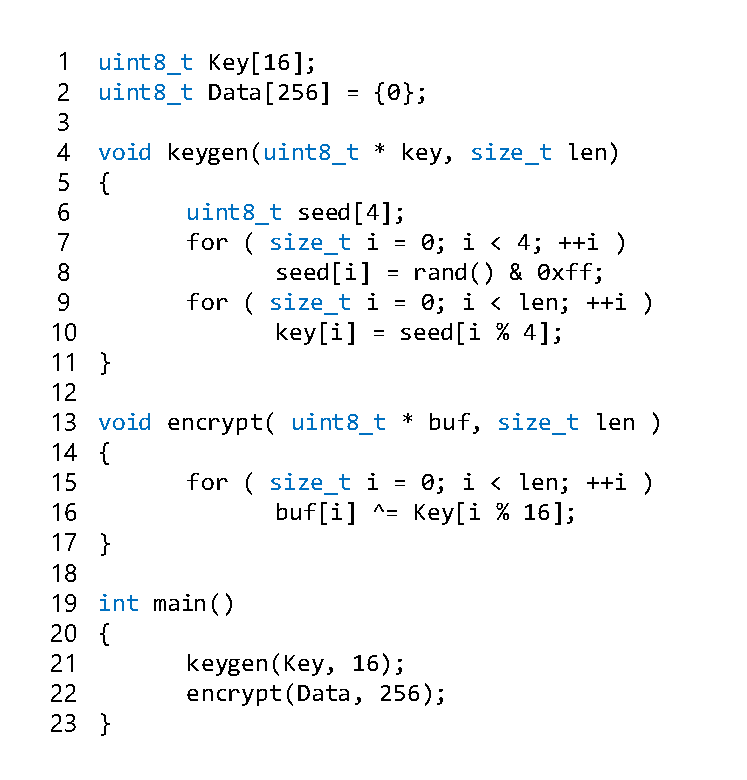
\includegraphics[width=0.4\textwidth]{code.pdf} \label{fig:dd:code} }

\subfloat[Partial corresponding disassembly code]{ 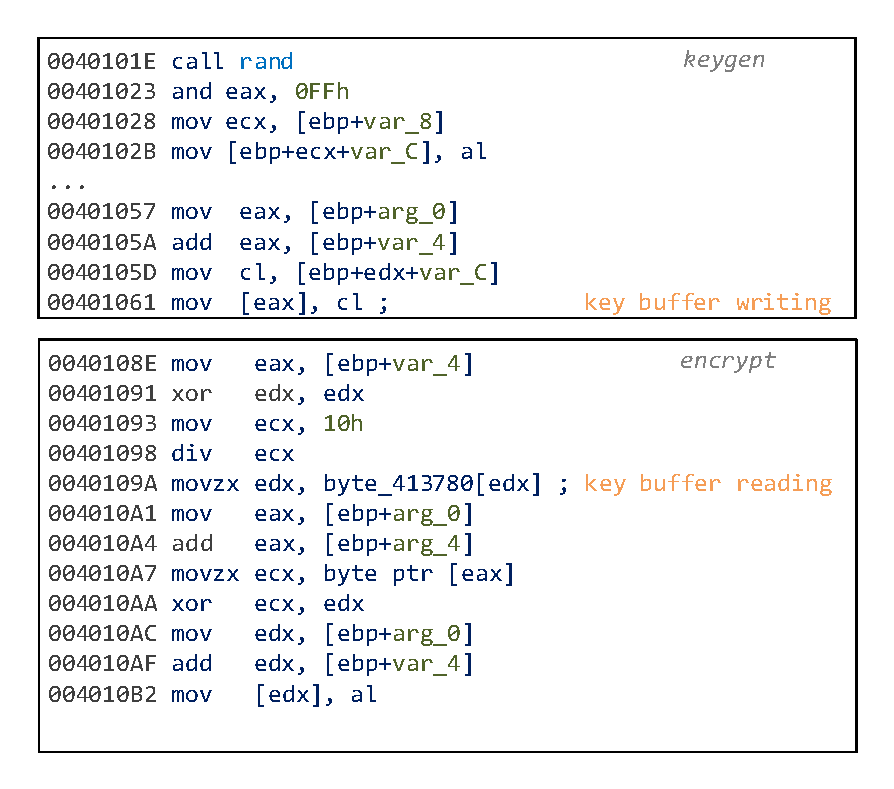
\includegraphics[width=0.4\textwidth]{depend.pdf} \label{fig:dd:asm} }
%
\caption{An example illustrating typically how a crypto key is used in a binary executable.}
\label{fig:dd}
\end{figure}

%\vspace{-0.15in}
%\paragraph{A Running Example} 
We use a simple but representative program, illustrated in~\autoref{fig:dd}, to demonstrate how our insecure crypto key detection works. 
This simple program encrypts \texttt{Data} 
%(defined at line 2 at Figure~\ref{fig:dd:code}) 
through masking a \texttt{Key} generated by the \texttt{keygen} function. 
The program captures a crypto operation (a simple cipher that mixes \texttt{Key} and \texttt{Data}) and a crypto key management (a home-made key derivation that generates a random key). 
{It has an insecure crypto key because 1) the key only contains four bytes of randomness and 2) the key is not sanitized after the encryption}.

To detect the insecure crypto key in this running example, a security analyst would need to 
(1) find which code blocks are crypto related; 
(2) identify the crypto key used by those blocks; 
(3) check how the identified crypto key is generated, i.e., which data sources affect it and how it is derived from those key materials; and
(4) monitor key propagation (i.e., the memory buffers that store the key) to check whether it is still available after the crypto operation. 
\sysname is designed to automate these steps with a principled approach. 

\paragraph{Challenges} 
To detect insecure keys using the above steps, our approach needs to address the following challenges:
\begin{compactitem}
\item \textbf{How to identify crypto operations without signatures}. 
Previous works that analyze crypto software often rely on signatures for specific crypto algorithms. 
Thus, if the algorithm is proprietary, the identification would fail, as no signatures would typically be available. 
In Figure\autoref{fig:dd:code}, the simple, home-made crypto operation cannot be identified with signatures. 

\item \textbf{How to identify the crypto keys}.
Even when the crypto operation has been identified, how to accurately locate the memory buffer that contains the crypto key is still non-trivial. 
For instance, the \texttt{encrypt} function in Figure\autoref{fig:dd:code} accesses two buffers: \texttt{Data} and \texttt{Key}. 
Unfortunately, when analyzing binary executables, there is no semantic information available on the buffers. 
Thus, our approach must identify which buffer is the crypto key buffer. 

\item \textbf{How to detect insecure crypto keys in complex programs}.
Having identified the buffer holding a key, we still need to determine if the key is correctly derived and managed. 
Unfortunately, programs that contain crypto algorithms are often complex and these algorithms usually only occupy a very small percentage of the entire program. 
It is infeasible and ineffective to analyze the whole program executable. 
Thus, we have to design an efficient way for detecting insecure crypto keys.
\end{compactitem}

% \begin{figure*}[!htbp]
% \centering
% 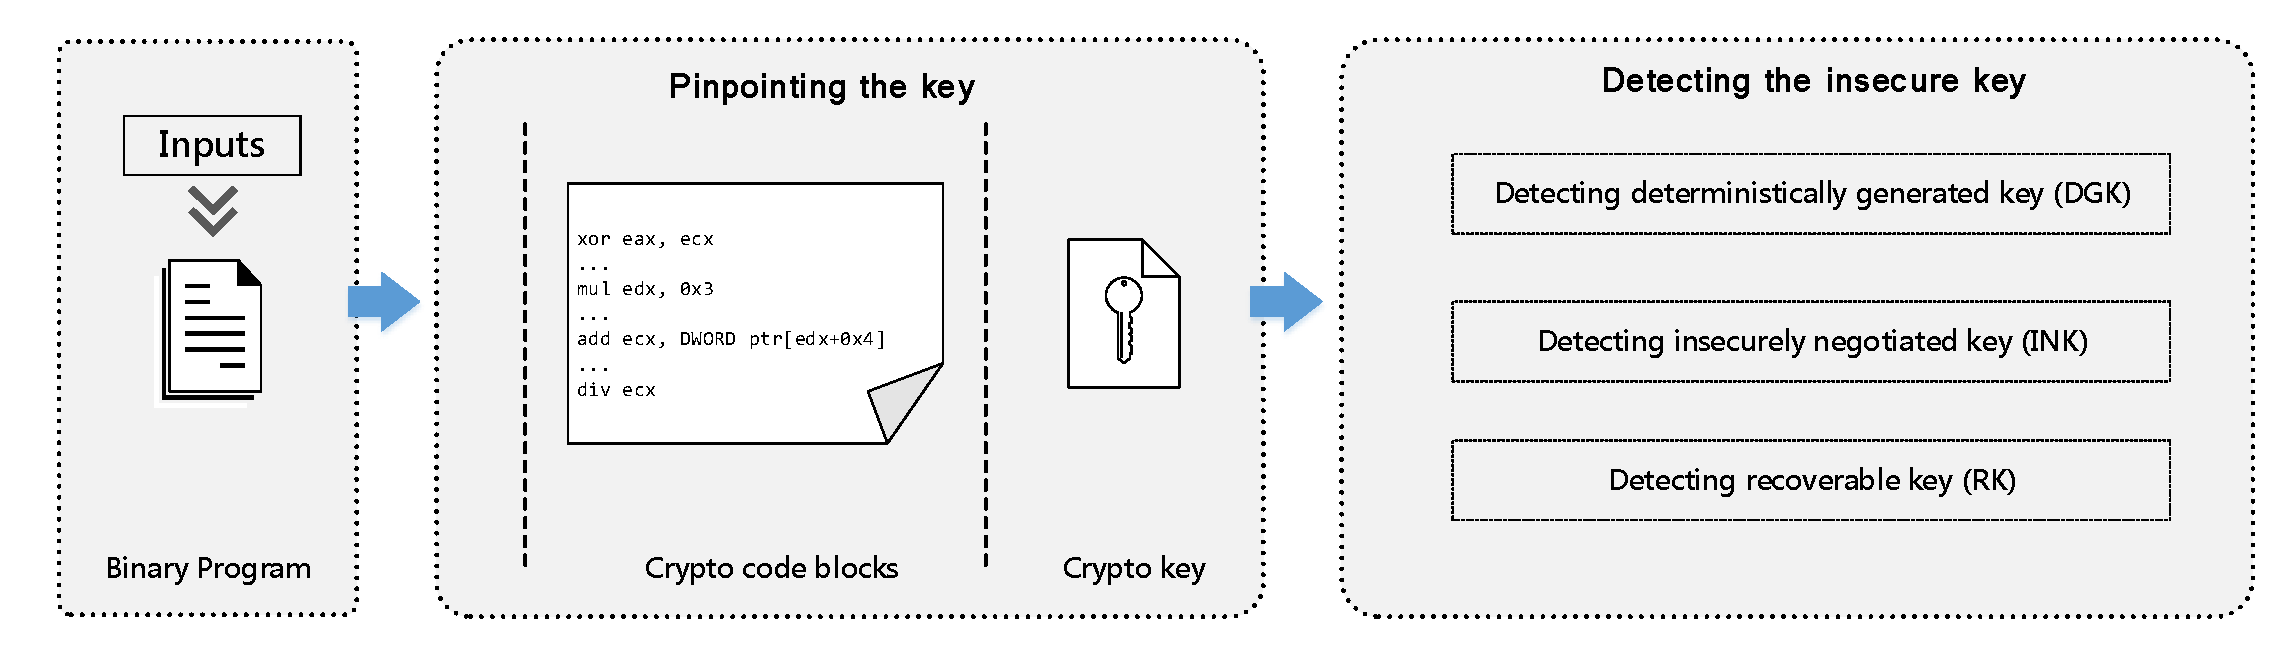
\includegraphics[width=0.9\textwidth]{flow.pdf}
% \caption{An Overview of \sysname.}\label{fig:workflow} 
% \end{figure*}


\paragraph{Insights} Fortunately, all of the challenges listed above can be solved with the following key insights:

\begin{compactitem}
\item
\textbf{Identifying crypto operations independent of their implementation}. 
Oftentimes, crypto operations are identified by scanning the implementation with signatures of well-known crypto algorithms. 
However, such approach cannot detect propietary algorithms.  
Instead, our approach identifies the {crypto basic blocks} at the core of the crypto operation. 
For this, it uses a dynamic analysis technique that leverages the insight that these core basic blocks usually mingle crypto keys and data, and thus have distinct properties. 
For instance, as shown in Figure~\ref{fig:dd:code}, the key masking operation (at line 16) reads from two data buffers and produces the ciphertext. 
Such crypto basic blocks have distinguishable properties such as high use of arithmetic instructions, producing data streams with high randomness, and having execution length proportional to the input size. 
If a basic block meets these three constraints, it is very likely that it is a crypto basic block.
% We can therefore rely on such features to find {crypto basic blocks} and further locate crypto keys. 
%We have to note that we are not the first to utilize this insight and it has been exploited before by Dispatcher~\cite{caballero2009dispatcher} and ReFormat~\cite{wang2009reformat}.

\item
\textbf{Locating the crypto keys}.
Once the core {crypto basic blocks} are identified, our approach then examines the data accessed by those blocks. 
Typically, {a crypto basic block} will process two inputs. 
For encryption, the plaintext and the key. 
For decryption, the ciphertext and the key. 
And, for digital signatures, the input message and the key. 
Note that while the verify function of a digital signature takes three inputs (message, key, signature), only the message and the key are used in the crypto operations.
Therefore, in all three cases we need to separate the crypto key from the other input. 
Interestingly, we notice that the size of the crypto key is usually very small (e.g., 128-bit) compared to the plaintext, ciphertext, or message, which could be of arbitrary length. 
We also observe that the crypto key and the other input are usually stored at different memory buffers. 
And, those buffers are usually filled with content derived from different data sources, e.g., a pseudo-random generator for keys and the network or the filesystem for the plaintext/ciphertext/message. 
%For instance, as shown in Figure~\ref{fig:dd:asm}, the operated crypto key and plaintext (line 7) depends on the memory writing operations at line 13 and 16, respectively. 

\item
\textbf{Detecting the insecure crypto keys}.
Since it is very complex to analyze the entire program to understand the handling of crypto keys, we instead propose a key-centric strategy. 
Having identified the crypto operations and located the crypto keys, we use the identified keys as an index to further check the origin of each key and its propagation. 
For instance, through checking the origin of the key in~\autoref{fig:dd} we can find that it is generated from the \texttt{keygen} function at line 10, {and through checking the input of this function we can discover the crypto key buffer contains inadequate information (i.e., only 32 bits) }.
Moreover, by monitoring the key buffer we can observe that its content is preserved until the program terminates, and thus it is an insecure crypto key. 
This backward and forward key tracking hence provides a simple way to detect insecure crypto keys.
\end{compactitem}


\paragraph{Problem Scope}
The objective of this work is to identify  insecure crypto keys in binary executables.
In particular, we focus on detecting (1) whether the key is generated from deterministic inputs, (2) whether a shared key is generated using key materials from a single party, and (3) whether the key is not sanitized immediately after the cryptographic operations. 
%
We focus on analyzing x86/64 stripped executables without source code or debugging symbols. 
%Particularly, we focus on both situations where cryptographic code is statically linked into a host program (thus the symbol names are removed) or dynamically invoked as an independent library (thus the symbol names are kept for dynamic linking). 
%With respect to the insecure crypto keys,
In addition, we focus on ciphers (symmetric, asymmetric, stream) and digital signatures. 
For these classes of cryptographic primitives, it does not matter which specific crypto algorithm the program uses.
Thus, our approach handles both standard and proprietary algorithms.
Other cryptographic primitives such as hash functions do not use keys, or in the case of keyed hashes they do not apply the crypto operations on the input and the key simultaneously.
% , thus violating our insights.


 
 
\section{Design}
\label{sec:solution}
\begin{figure*}[htbp]
\centering
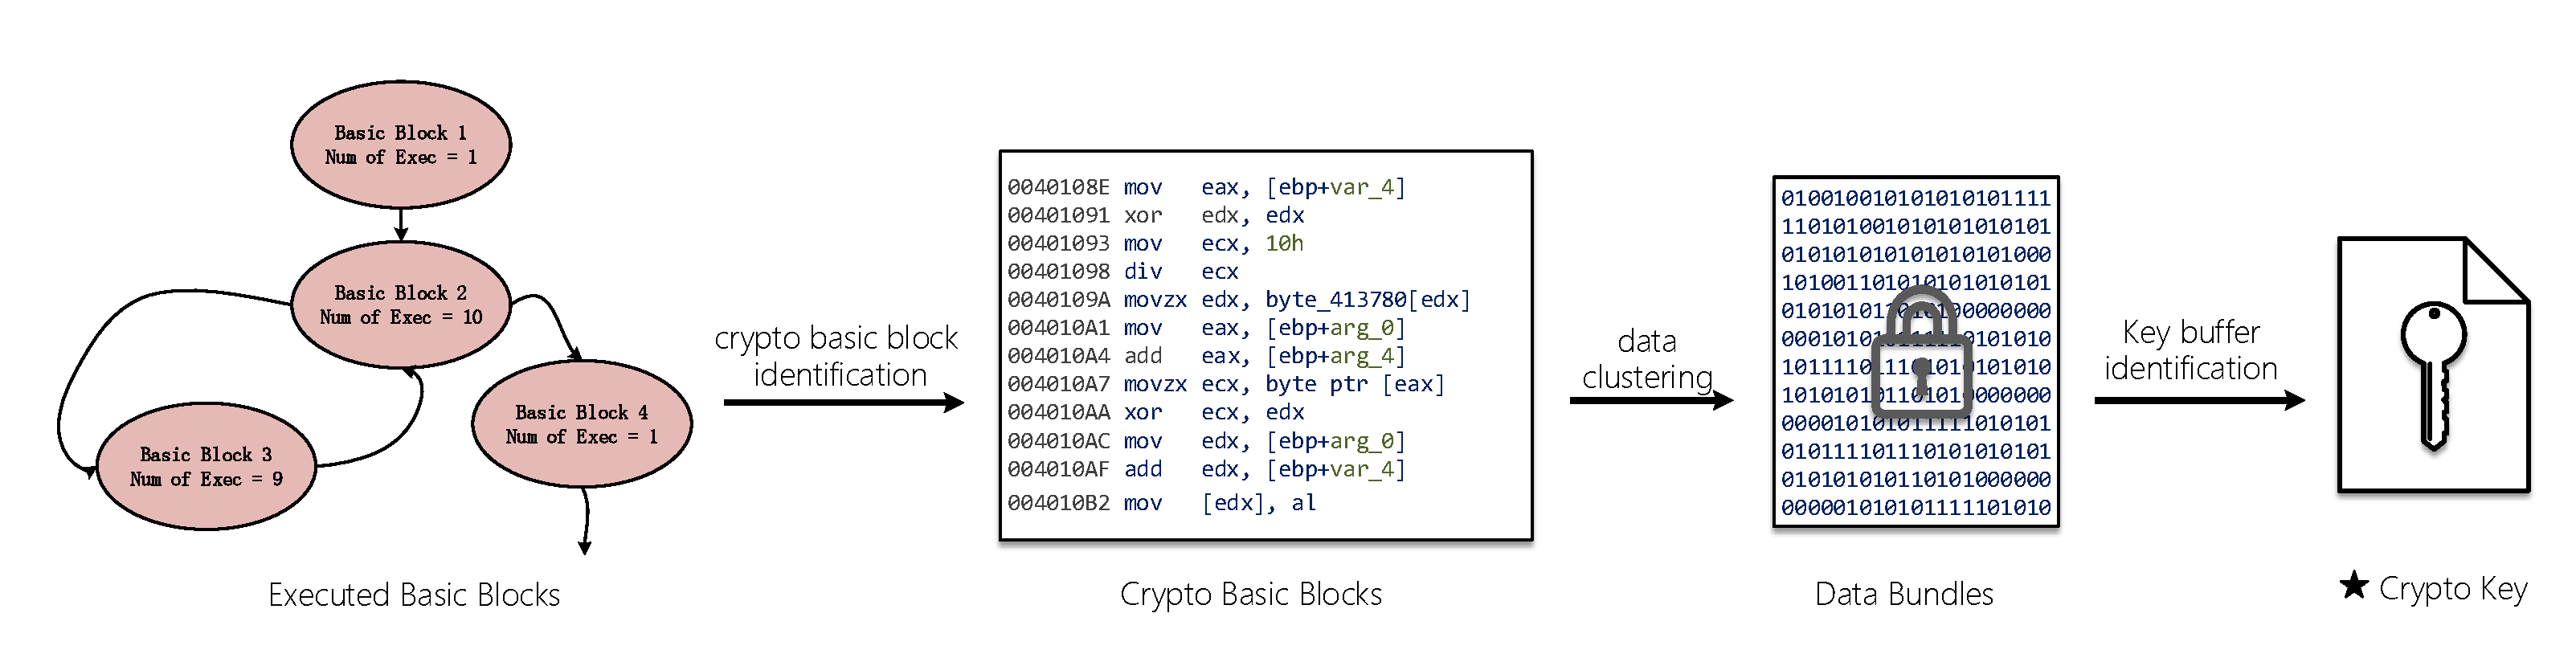
\includegraphics[width=\textwidth]{keyPinpoint.pdf}
\caption{The process of pinpointing crypto keys in binary executables\label{fig:cry} }
\end{figure*}

%An overview of \sysname is presented in~\autoref{fig:workflow}. 
\sysname uses dynamic analysis to identify insecure crypto keys. 
It assumes that there exist test cases to execute the program so that it uses the crypto operations. Our approach uses dynamic analysis because it needs statistics about the program execution.
%  randomness of the runtime data, and also the number of executions of basic blocks. 
Furthermore, static analysis faces many limitations for analyzing memory buffers, which store the crypto keys.
%
At a high level, \sysname comprises of two phases:

\begin{compactitem}

\item \textbf{Pinpointing the Key}. 
In the first phase, detailed in~\S\ref{sec:analysis:pinpoint}, the target program is executed with a lightweight coarse-grained  binary code instrumentation to firstly identify the crypto basic blocks and then identify the crypto keys they use.

\item \textbf{Detecting the Insecure Key}. In the second phase, detailed in~\S\ref{sec:analysis:misuse}, the target program is executed again with a heavyweight  fine-grained  instrumentation, which tracks the memory reads and writes and conducts a function level taint analysis. 
% with the user or system generated input. 
Through taint analysis of the pinpointed keys, \sysname then detects the insecure crypto keys. \looseness=-1

\end{compactitem}


\subsection{Pinpointing Crypto Keys}\label{sec:analysis:pinpoint}

The first phase of \sysname is to pinpoint the crypto keys. 
An overview of how \sysname performs this analysis is presented in~\autoref{fig:cry}. 
%We define a crypto operation as the set of crypto basic blocks executed during a specific application (e.g., an HTTPS communication).
It first identifies the crypto basic blocks by running the executable with multiple test inputs, and then analyzes the data those basic blocks operate on to locate the crypto keys. 
% Consequently, this analysis consists of two steps: (i) crypto basic block identification, and (ii) crypto key buffer identification.

\paragraph{Step-I: Crypto {Basic Block} Identification} % \label{sec:analysis:pinpoint:locate}
One observation of modern crypto algorithms (e.g., \textsf{\small AES}, \textsf{\small RSA},  \textsf{\small DSA}) is that they are typically built with only a few compact transformations, which correspond to just a few basic blocks in a program. 
Therefore, if we can identify these basic blocks, we would  identify the crypto operations that use them. 
% To achieve this, we leverage a number of common features to identify a crypto basic block. 

\begin{Definition}
\label{def:cryptoblock}
A crypto basic block is defined as a basic block that satisfies the following constraints: 
(i) the basic block uses arithmetic calculations to implement a cryptographic  operation; 
(ii) the basic block is executed multiple times to mix a data stream with a key stream; 
%(iii) the produced (or consumed) data should have both high entropy and high randomness.
(iii) the produced or consumed data have high randomness.
% that reflect strong cryptographic features such as frequently using arithmetic instructions and producing highly random data.
\end{Definition}

Our approach first computes, for each basic block, the ratio of  x86/64 arithmetic and bitwise instructions (e.g., \texttt{mul}, and \texttt{xor})~\cite{caballero2009dispatcher, intelx86}. 
A basic block is considered a candidate crypto basic block if it has a ratio larger than a pre-defined threshold. 
This threshold has been experimentally selected as 15\% in our current design after analyzing common crypto libraries and utilities.
A special case is that a basic block is directly considered a candidate if it contains instructions from the Advanced Encryption Standard instruction set (AES-NI),  an extension to the x86 instruction set for microprocessors from Intel and AMD.

Next, it checks whether the candidate basic blocks are \emph{data sensitive}. 
A basic block is data sensitive if the total amount of execution for the basic block is proportional to the size of its input data. 
We prepare four test suites with inputs of different size magnitude to test the program, and calculate for each candidate basic block, 
the total number of executions of the basic block across all inputs, the total basic block's input data size, and the total basic block's output data size. 
Candidate basic blocks for which the number of executions increases approximately linearly with the ratio of input/output data size are kept as candidate crypto basic blocks. Other candidates are discarded.
 
At this point, our approach has checked the first two conditions  in Definition~\ref{def:cryptoblock}. 
The last condition checks if the data operated on by the candidate basic block has high randomness. 
However, each time a basic block is executed it only operates on part of the input data. 
Thus, our approach accumulates all the data that each candidate basic block operates on during the entire program execution into data bundles.

\begin{Definition}
A data bundle is defined as the sequence of all the data that an operand of an instruction operates on during the entire execution of the program. The size of a data bundle is the number of data items it contains.
\end{Definition}

{For example, in Figure~\ref{fig:dd:asm} the instruction at \texttt{0x0040109A} has one memory read operation and is executed 256 times. Therefore, there will be a data bundle with 256 data items: the sequence of value read that is from \texttt{byte\_413780[edx]}.
% and the sequence of value write that is to \texttt{edx}.} \ZQ{not clear to me. Since this is written to register edx, why there is a bundle?}
%
Our approach focuses on data bundles that are generated by  instructions with memory operands, since registers have a limited size that does not typically hold a crypto key.
%We search for high entropy data among all data bundles. 
Once the data bundles are built, they are examined to identify those that contain highly random data. 
%Interestingly, many other data transformations (especially data compression) could also generate data of high entropy. 
%Hence, we should further distinguish crypto operations from other data encoding operations. 
%Fortunately, while data encoding operation may generate data of high entropy, the randomness of crypto data is actually distinguishable~\cite{wang2013steal}. 
%From this point of view, if a bundle has high-entropy, it is checked using an in-depth data randomness analysis with \emph{Chi-Square distribution} and \emph{Monte Carlo} $\pi$ \emph{approximation} tests. 
For this, {our approach leverages the \textsf{\small ent}~\cite{ent_random} utility to measure the randomness of the collected data bundle with both \emph{Chi-Square distribution} and \emph{Monte Carlo} $\pi$ \emph{approximation} tests}.
If \textsf{\small ent} judges the data bundle as random, the candidate basic block is considered a crypto basic block.

In our running example in Figure~\ref{fig:dd:asm}, the basic block (\texttt{0x0040108E}-\texttt{0x004010B2}) is the crypto basic block to be identified.
It satisfies the above constraints for a crypto basic block:
	it utilizes arithmetic and bitwise instructions to implement the crypto operation, 
	the number of executions of the basic block is proportional to the size of the input data, 
	it accesses several memory buffers, and its produced data has high randomness.

\paragraph{Step-II: Crypto Key Buffer Identification}
Having identified the crypto basic blocks in Step-I, our approach next identifies the crypto keys used by those basic blocks. 
Different types of data may be handled by a crypto basic block: crypto key, plaintext, ciphertext, and message to be signed. 
More concretely, a crypto operation will take two inputs: 
crypto key and plaintext for encryption, 
crypto key and ciphertext for decryption, and 
crypto key and message for digital signature. 
Thus, the crypto key should always be an input to the crypto basic block. 
Therefore, we can exclude the data output by the crypto basic block and just focus on the input data. 
Still, our approach has to separate the crypto key from the other input. 
And, it  can no longer use randomness for this since both the crypto key and the ciphertext will have high randomness.

\begin{Definition}
A crypto buffer is defined as all operated memory addresses in one data bundle of a crypto basic block,
and the size of a crypto buffer is the number of unique memory addresses it contains. 
\end{Definition}

{For instance, the memory read data bundle of the  instruction at \texttt{0x0040109A} in Figure~\ref{fig:dd:asm} contains 256 items.
This bundle, however, only contains 16 unique memory addresses, thus the size of corresponding crypto buffer is 16 instead of 256.
When we test the randomness of the data, we use the concept of bundle because a buffer may be accessed randomly and we should concern about the access sequence.
If the high randomness is discovered, we then only concern about the range of accessed memory,
	and thus we use the concept of buffer to help distinguish key from data.
}

To identify which input is the crypto key buffer, \sysname leverages the following two complementary insights.

\begin{compactitem}
\item \textbf{Using the buffer size}. 
Typically, the crypto key buffer is small compared to the ciphertext/plaintext/message buffer: a key can be stored in a relatively small buffer but the crypto input often needs a larger memory buffer. 
This feature becomes even more obvious when executing the crypto basic blocks with multiple inputs: either the key is repeatedly used or it is updated between different iterations (e.g., the state update of a stream cipher), and the key is generally stored in a fixed-length memory buffer whereas the length of the ciphertext/plaintext/message varies according to the size of the program input.
% Please note that we can test the program with inputs of different sizes, or execute the program repeatedly  to observe the variation of the input buffer, and exclude those non-key buffers.}

\item \textbf{Using the execution context}.
The other insight is that crypto keys and other input data are typically initialized by different functions. 
If we track the execution context of how the data is initialized, we can easily differentiate them as well. 
For instance, the used crypto key buffer is usually initialized by a key derivation function or from a pseudo-random number generator, while the plaintext/ciphertext/message is generally directly read from a file or network socket. 

\end{compactitem}


\subsection{Detecting Insecure Keys}
\label{sec:analysis:misuse}

The second phase of \sysname detects the insecure crypto keys. 
Unlike the first phase where we perform a lightweight dynamic binary analysis to collect execution statistics (e.g., the number of executions for a basic block and the randomness of data bundles), the second phase requires a heavyweight dynamic binary analysis to trace how keys are generated and propagated.
At a high level, our analysis is a function-level variant of dynamic taint analysis (e.g,.~\cite{song2005ndss, schwartz2010oakland}) with the following taint policies. \looseness=-1

\paragraph{Taint Sources} 
\sysname uses three different taint tags to capture whether a value has been derived from a local input  (i.e., filesystem or return value from the \texttt{rand} function), a remote input (i.e., the network), or 
none of those two (i.e., deterministic value). 
Thus,  each memory location (i.e., byte) in the shadow memory~\cite{schwartz2010oakland} has a two-bit taint tag with values 00 for no input, 01 for local input, and 10 for remote input.  
At initialization, all memory locations will be assigned the no-input tag. 
During program execution, if \sysname observes that a memory location is assigned from local input (remote input), \sysname assigns the local (remote) taint tag to the memory location. 
For instance, \texttt{Key} at line 13 in our running example in Figure~\ref{fig:dd:code} will be assigned with a local input tag. 


In addition, to quantitatively measure how many of bytes of information generated for crypto keys, we introduce the concept of the length of input for the buffer involved for key generation.
\begin{Definition}
The input length (IL) of a buffer is the number of bytes derived from program inputs.
\end{Definition}
\noindent
For instance, in our running example the \texttt{keygen} function initializes four bytes of the \texttt{seed} buffer using function \texttt{rand}. Then \sysname keeps a 4-byte IL for this buffer.


\paragraph{Taint Propagation} \sysname could use a fine-grained taint analysis (e.g.,~\cite{song2005ndss}) to trace each instruction and propagate the taint tags correspondingly. 
However, we found such an approach often incurs high performance overhead to the analyzed program, e.g., causing a remote peer to close the network socket due to connection time out, or the GUI freezing for non-networking programs, e.g., \textsf{\small WinRAR}. 
Therefore, we have develop a lightweight, function-level, taint propagation policy, which propagates  taint tags based only on the memory read and memory write operations inside the execution context of a function.
This propagation is based on the fact that \sysname only requires knowing whether a buffer contains data from either deterministic, local input, or remote input (i.e., the three taint tags). 
Therefore, it does not need to propagate the taint tags precisely for each instruction. 
Instead, it can propagate taint tags at the higher function level, significantly improving efficiency.

More specifically, \sysname taints all the data definitions (i.e., memory writes) inside a function using the taint tag of the input data. 
% (i.e., determined by the memory read instructions) to this function. 
As such, it only needs to instrument the memory read and write instructions. 
The memory read instructions define the taint source for the function, and the memory write instructions define the taint tags for the memory data based on the current function's taint . 
If a new taint source to the function is observed, the new taint tags are unioned with the current function's taint tag. All the defined data inside this function will from that point on have a unioned taint tag (e.g., tag with bits 11 to represent both local and remote input). 
In our running example, the \texttt{seed} buffer in the \texttt{keygen} function  will be tainted with local input tag, and thus the global \texttt{Key} buffer will also be assigned the local input tag. 
% Note that the reason of why we are only concerned with memory data (register data is not included) is because crypto keys usually have a larger length (e.g., at least 128 or 256 bits, etc.) and typically cannot be hold by registers. 




%\review{In addition, to quantitatively measure the randomness of the information contained in a buffer, we define the IL of a buffer as the bytes directly derived from program inputs or indirectly transferred from other buffers.
%For instance, in our running example the \texttt{keygen} function initializes four bytes of the \texttt{seed} buffer using \texttt{rand}. Then \sysname keeps a 4-byte IL for this buffer.
%}

{
While propagating the taint tags, we also propagate the IL for the buffers. Such information is particularly useful for determining whether a key has sufficient randomness. In particular, for each function, \sysname tracks the total number of IL. Then whenever there is a memory write information, it propagates the current IL to this buffer. When the function returns, it recalculates the IL for each buffer based on both the number of bytes accessed and also the current IL for this function. 
% If a buffer is not directly initialized by the program input, \sysname assigns an IL to it according to all accessed intermediate buffers in a function.
% To implement this, \sysname keeps tracking the buffer accessed by one function as soon as it starts executing. 
Assume that one function accesses two buffers during its execution.
\sysname records how many bytes in each buffer are accessed, respectively.
If the number of bytes does not exceed the IL of the host buffer,
	\sysname adds this number to the IL of the newly initialized buffer.
Otherwise it adds the IL of the host buffer to the IL of the new buffer.
Finally, we check whether the IL of the new buffer is larger than the size of the buffer.
If so, the IL is adjusted to the size of the buffer.
Through performing such IL propagation, \sysname maps the information from input buffer to the output buffer of one function.
 }

% \ZQ{shall this paragraph go to the taint source? when we taint the source of input, we also track the input length when we see such input?}

% \ZQ{In the taint propagation, we need to track the size of input length for a buffer.}


\paragraph{Taint Sinks} With the aforementioned taint sources and taint propagation policy, all the memory locations will have a taint tag showing whether the data comes from local or remote input, or is deterministic. 
To identify insecure crypto keys, 
\sysname checks the taint tag of the buffer at the crypto basic block (to check whether the key is improperly generated) or when the program exits (to check for key residue). 
In particular, we use the following policies to detect the insecure crypto keys.

\begin{compactitem}
\item \textbf{Detecting DGK}. 
If a key is not derived from any input, i.e., is deterministic,  
then \sysname considers that the generation of the key is flawed.
{
In addition, \sysname checks whether the key receives enough information from non-deterministic inputs.
This is done through an analysis of the key buffer IL.
For example, in our running example the key is initialized in the \texttt{keygen} function.
At the beginning of the function a \texttt{seed} buffer is initialized with a 4-byte IL.
Then the \texttt{key} buffer in the same function is initialized.
At that time, the IL of the \texttt{key} buffer is also assigned as 4 because the function only accesses one buffer with a 4-byte IL.
As a result, even if the size of the \texttt{key} buffer is 16, it has a smaller IL of 4-byte.
Eventually, if the IL of a key buffer has the size less than a threshold, 16 bytes (128 bits) in our current design, we consider the key is insecure.
In this case the used key buffer has a 4-byte IL and is obviously insecure.
}

% In our running example, the length of the key is actually 16 bytes, which will be detected insecure by \sysname.

%\ZQ{it is not clear how the length of the IL is computed. What do you mean the sum of these two IL? What do you mean the actual size? Maybe give an example}

%\JR{The example is provided, and since the size of used key in our running example equals to 16 bytes, we do not consider it an insecure one.}

\item \textbf{Detecting INK}. 
An insecurely negotiated key is a crypto key shared between two parties (e.g., a session key between a client and a server) where the key value is only influenced by one party~\cite{keyValidated2017}. 
{A negotiated key is the symmetric key used for encrypting or decrypting network data.}
If we know there is a negotiated key but the taint tag for this key includes only local input tag or remote input tag (not both), \sysname considers this is an insecurely negotiated key. \looseness=-1

\item \textbf{Detecting RK}. 
When a crypto operation terminates, all memory buffers holding involved crypto keys should be cleared~\cite{yang2017dead}. 
%Since we have located the keys and tracked their propagation (even though this is at a coarse granularity), 
To detect any recoverable keys, 
\sysname searches the memory to check any partial existences of the keys in memory 
when the process terminates. 
A key is considered recoverable if one third of its content still exists in memory~\cite{heninger2009reconstructing}. 
Therefore, we cross check the content of the data bundles, and if one third of the content still matches with the original key buffer, \sysname considers it a recoverable key. 
{In our running example, the \texttt{Key} buffer is allocated in the global memory region, and is not cleared after process termination. \sysname therefore detects it is an RK case.}

\end{compactitem}



 

\section{Implementation}
\label{sec:kxray}
%\vspace{-0.12in}
%\paragraph{Dynamic Binary Code Analysis} 
We have implemented \sysname using  Intel \textsf{\small PIN}~\cite{luk2005pin}, 
a popular dynamic binary instrumentation (DBI) framework. 
We use dynamic analysis instead of static analysis for different reasons. 
First, we need to measure execution statistics such as the randomness of the runtime data and the number of executions of a basic block. 
Second, static analysis faces limitations analyzing memory buffers, e.g., due to indirect memory addressing.
Third, the static dentification of function boundaries, 
needed for the function-level taint propagation, is challenging, especially for C++ libraries~\cite{andriessedepth}. 
Using DBI, \sysname can leverage the runtime information to identify function boundaries. 
Finally, DBI is able to handle executables with some protections (e.g., code packing or VM obfuscation). \looseness=-1

% \sysname contains two phases of analysis with different instrumentations, and 
We have implemented three Pintools for \emph{code profiling}, \emph{randomness testing}, and \emph{key tracking}. 
In Phase I, the executable is first run with the code profiling Pintool to find which candidate basic blocks should be tested for randomness. 
Then, the program is executed again with the randomness testing Pintool to collect the runtime information needed for the randomness test.
In Phase II, the key tracking Pintool is used to check how program inputs affect the key derivation and how crypto keys are propagated.

To detect the key residue, we should rigorously have implemented a kernel module to monitor all of the process pages belonging to the target process right after the process terminates. 
Unfortunately, PIN does not provide such kernel-level APIs. 
Instead, we instrument the callback function \texttt{PIN\_AddFiniFunction} in our key tracking pintool to trigger the memory check. 
This callback is invoked right after the execution of all user defined cleanup functions and before the process terminates.

\paragraph{Labeling Program Inputs} \sysname needs to set the input taint tag when the program receives  local or remote input. To this end, it hooks the system APIs that deal with such inputs (e.g., \texttt{read}, \texttt{fread}, \texttt{recv}) , as well as APIs related to random number generation (e.g.,  \texttt{rand()}).
The local tag is set if the input comes from the filesystem or a random number generation API, 
and the remote tag if the input comes from a network socket.
% A special case is how to recognize the pseudo random number generator (PRNG). A PRNG often combines multiple system input sources to produce pseudo random stream.
% We found that if we directly hook every system input and check for combinations to identify a potential PRNG, the analysis will be very complex. 
% Fortunately, we find that the implementations of PRNG in real world are often provided by the operating systems or widely used crypto libraries. 
% Thus, we collect the features of well-known PRNGs beforehand. When our analysis encounters such a PRNG, it can be identified straightforwardly using a feature matching.

\paragraph{Differential Testing}
%Since crypto basic blocks are only a very small fraction of all basic blocks, 
\sysname can optionally use a differential analysis step to identify candidate basic blocks in Phase I that are unrelated to crypto operations, and thus be removed from the candidate set. 
To this end, it compares two traces, obtained by running the program executable with and without triggering the crypto operations (e.g., executing \textsf{\small 7-zip} with or without file encryption). 
Then, it identifies candidate basic blocks that do not appear in the execution with crypto operations, as well as candidate blocks that apper in both executions with and without crypto operations. 
In both cases, those candidate basic blocks cannot be crypto basic blocks. 
Note that differential analysis is just an optional optimization to reduce the number of candidate basic blocks to be considered.

\paragraph{On-Demand Tracing}
Crypto operations are often CPU-intensive and a dynamic analysis with large performance overhead could significantly interfere with the normal program execution. 
To address this, \sysname uses on-demand tracing , applying heavyweight program analysis only on necessary code blocks. 
For instance, in the first phase, both the number of executions of candidate basic blocks and the data randomness are analyzed to determine the crypto basic blocks. 
However, the testing of randomness requires a time-consuming analysis. 
To reduce this overhead, \sysname first uses code profiling to count the number of candidate basic block executions and excludes irrelevant candidate basic blocks. 
In this manner, it only needs to apply the more expensive randomness testing on the remaining candidate basic blocks. 
In the second phase of analysis, \sysname only instruments the memory read and memory write instructions to propagate the taint tag at function level, as described in \S\ref{sec:analysis:misuse}. This significantly reduces the overhead of our taint analysis.

\paragraph{Entropy Test}
A time-consuming step in \sysname is the randomness test.
To speed this step, we conduct a more lightweight entropy test before, so that the randomness test is only applied to those bundles with high entropy. 
Note that a bundle with high randomness must also possess high entropy, while a bundle with high entropy may not have high randomness~\cite{wang2013steal}.

%\paragraph{Optimizations with Special Crypto Implementations}
% Although our crypto block identification technique requires no priori knowledge of a crypto algorithm, we also consider two special cases. 
% The first case is the AES New Instructions (\textsf{\small AES NI}) introduced by Intel to accelerate the encryption. 
% When encountering such instructions, we directly extract the \textsf{\small AES} keys based on the semantics.
% The second case is the crypto APIs provided by crypto libraries or the operating systems. 
% These APIs can be identified easily through checking the names. 
% Note that we handle these specific implementations just for optimization purposes and \sysname does not have to rely on them when analyzing a target binary. \looseness=-1

\paragraph{Online Analysis}
\sysname uses an online analysis approach.
It could also operate on execution traces to reduce the runtime overhead. 
Nonetheless, we found an online approach is more suitable to our goal because offline analysis leads to extremely large execution traces (often >100GB), which create an I/O bottleneck slowdown.



\section{Evaluation}
\label{sec:evaluation}
\begin{table}[t]
\scriptsize 
\centering
\begin{tabular}{p{2cm} p{0.8cm} p{2.1cm} p{1.5cm} }
\toprule
\textbf{Library}						& \textbf{Version}	& \textbf{Category}		& \textbf{Protection} \\ 
\midrule
{Botan~\cite{botan_cryptozoo}}				& {1.10.13}			& {Crypto Libraries}		& - \\
{Crypto++~\cite{cryptopp_cryptozoo}}		& {5.6.4}			& {Crypto Libraries}		& - \\
{Libgcrypt~\cite{libgcrypt_cryptozoo}}		& {1.6.6}			& {Crypto Libraries}		& - \\
{LibSodium~\cite{libsodium_cryptozoo}}		& {1.0.12}			& {Crypto Libraries}		& - \\
{LibTomcrypt~\cite{libtomcrypt_cryptozoo}}	& {1.17}			& {Crypto Libraries}		& - \\
{Nettle~\cite{nettle_cryptozoo}}			& {3.3}				& {Crypto Libraries}		& - \\
\midrule
{GnuTLS~\cite{gnutls_cryptozoo}}			& {3.5.13}			& {SSL/TLS Libraries}		& - \\
{mbedTLS~\cite{mbedtls_cryptozoo}}			& {2.3.0}			& {SSL/TLS Libraries}		& - \\
{OpenSSL~\cite{openssl_cryptozoo}}			& {1.1.0f}			& {SSL/TLS Libraries}		& - \\
{WolfSSL~\cite{wolfssl_cryptozoo}}			& {3.9.10}			& {SSL/TLS Libraries}		& - \\ 
\bottomrule
\toprule
\textbf{Application}					& \textbf{Version}	& \textbf{Category}		& \textbf{Protection} \\ 
\midrule
{7-Zip~\cite{7zip_cryptozoo}}				& {9.20}			& {File Compressor}			& - \\
{Ccrypt~\cite{ccrypt_cryptozoo}}			& {1.10}			& {File Encryptor}			& UPX \\
{Cryptcat~\cite{cryptcat_cryptozoo}}		& {1.2.1}			& {Messenger}				& - \\
{Cryptochief~\cite{cryptochief_cryptozoo}}	& {1.337}			& {File Encryptor}			& - \\
{Enpass~\cite{enpass_cryptozoo}}			& {5.6.0}			& {Password Manager}		& - \\
{Imagine~\cite{imagine_cryptozoo}}			& {1.1.0}			& {Picture Browser}			& UPX \\
{IpMsg~\cite{ipmsg_cryptozoo}}				& {4.60}			& {Messenger}				& - \\
{KeePass~\cite{keepass_cryptozoo}}			& {1.34}			& {Password Manager}		& - \\ 
{MuPDF~\cite{mupdf_cryptozoo}}				& {1.11}			& {PDF Parser}				& - \\
{PSCP~\cite{putty_cryptozoo}}			& {0.62}			& {SSH client}				& - \\
{Sage~\cite{sage_cryptozoo}}				& {2.0}				& {Ransomware}				& - \\
{Ultrasurf~\cite{ultrasurf_cryptozoo}}		& {15.04}			& {Proxy client}			& Themida \\
{WannaCry~\cite{wannacry_cryptozoo}}		& {1.0}				& {Ransomware}				& Dynamic DLL \\
{Wget~\cite{wget_cryptozoo}}				& {1.11.4}			& {Downloader}				& - \\
{WinRAR~\cite{winrar_cryptozoo}}			& {5.40}			& {File Compressor}			& - \\
\bottomrule
\end{tabular}
\vspace{0.1cm}
\caption{The collected binary executables in our benchmark.}\label{tab:cryptozoo}
\end{table}


    \begin{table}[t]
\scriptsize 
\centering

%\vspace{-0.55in}
%\vspace{-0.4in}
\scalebox{1}{
\begin{tabular}{l l c c c c c ccc}

\toprule
\textbf{Target} & \textbf{Algorithm} & \textbf{B1} & \textbf{B2} & \textbf{B3} & \textbf{N} & \textbf{S} & \textbf{IL} \\
\hline 
\multirow{4}{*}{Botan}		& AES-256			& 53 & 13 & 7			& 1 & 240 & 32 \\
							& RSA-2048			& 1180 & 569 & 162		& 6 & 1024 & 256 \\
							& ECDSA	& 958 & 921 & 300		& 2 & 224 & 128 \\
\midrule                            
\multirow{4}{*}{Crypto++}	& AES-256			& 1281 & 26 & 5			& 1 & 240 & 32 \\
							& RSA-2048			& 1949 & 924 & 214		& 6 & 896 & 256 \\
							& ECDSA	& 1916 & 1425 & 305		& 8 & 288 & 64 \\
\midrule
\multirow{4}{*}{Libgcrypt}	& AES-256			& 126 & 25 & 3		& 1 & 240 & 32 \\
							& RSA-2048			& 565 & 463 & 153	& 6 & 896 & 896 \\
							& ECDSA	& 340 & 322 & 49	& 10 & 320 & 96 \\
\midrule
\multirow{2}{*}{LibSodium}	& AES NI-256		& 7 & 4 & 4			& 1 & 240 & 32 \\
							& Ed25519			& 690 & 686 & 171	& 8 & 288 & 256 \\
\midrule
\multirow{4}{*}{LibTomcrypt}	& AES-256			& 60 & 43 & 4		& 1 & 240 & 32 \\
							& RSA-2048			& 404 & 385 & 69	& 7 & 1152 & 1152 \\
							& ECDSA	& 330 & 274 & 72	& 4 & 128 & 97 \\
\midrule
\multirow{4}{*}{Nettle} 	& AES-256				& 38 & 13 & 3		& 1 & 240 & 32 \\
							& RSA-2048				& 411 & 87 & 61		& 6 & 1152 & 896 \\
							& ECDSA		& 186 & 92 & 39		& 8 & 288 & 32 \\
\midrule
\midrule
\multirow{4}{*}{mbedTLS}	& AES-256			& 44 & 40 & 13		& 1 & 240 & 32 \\
							& RSA-2048			& 154 & 138 & 39	& 12 & 1664 & 256 \\
							& ECDSA	& 255 & 245 & 47	& 9 & 384 & 64 \\
\midrule
\multirow{4}{*}{OpenSSL}	& AES-256			& 58 & 10 & 4		& 1 & 240 & 32 \\
							& RSA-2048			& 210 & 175 & 41	& 10 & 1552 & 640 \\
							& ECDSA	& 188 & 143 & 17	& 6 & 192 & 50 \\
\midrule
\multirow{4}{*}{WolfSSL}	& AES-256			& 50 & 36 & 4		& 1 & 240 & 32 \\
							& RSA-2048			& 295 & 235 & 36	& 7 & 1152 & 1152 \\
							& ECDSA	& 277 & 202 & 27	& 5 & 160 & 32 \\
\midrule
\midrule
7-zip						& AES NI-256		& 2 & 2 & 2	 		& 1 & 240	& 32 \\
\midrule
Ccrypt 						& AES-256			& 44 & 5 & 1	 	& 1 & 240	& 32 \\
\midrule
Cryptcat					& Twofish			& 54 & 14 & 7		& 1 & 160	& varied \\
\midrule
Cryptochief 				& Proprietary $\ast$	& 23 & 12 & 1		& 1 & 8		& 3 \\
\midrule
Enpass 						& AES NI-256		& 8 & 3 & 3	 		& 1 & 240	& 32 \\
\midrule
Imagine						& DSA-1024 $\ast$	& 241 & 72 & 12	 	& 5 & 464	& 928 \\ % should be 464 == 128*3 + 40*2!!!
\midrule
IpMsg						& AES-256			& 168 & 12 & 4		& 1 & 240	& 32 \\
\midrule
Keepass						& AES-256			& 481 & 118 & 19	& 1 & 240 & 32 \\
\midrule
MuPDF						& AES-128			& 262 & 46 & 4	 	& 1 & 176	& 16 \\
\midrule
PSCP						& AES-256			& 195 & 9 & 5		& 1 & 240	&  32 \\
\midrule
Sage						& ChaCha20 $\ast$	& 31 & 17 & 2		& 1 & 256	& 32 \\
\midrule
UltraSurf					& RC4 $\ast$		& 191 & 79 & 6		& 1 & 1024 & 16 \\
\midrule
WannaCry					& AES-128 $\ast$	& 26 & 12 & 3	 	& 1 & 352	& 16 \\
\midrule
Wget						& AES-256			& 268 & 22 & 3		& 1 & 240	& 32 \\
\midrule
\multirow{2}{*}{WinRAR} 	& AES-128 $\ast$	& 181 & 58 & 3		& 1 & 176	& 32 \\
 							& AES-256 $\ast$	& 214 & 51 & 3	 	& 1 & 240	& 48 \\
\bottomrule


% \multicolumn{7}{p{8.4cm}}{B1: the number of basic blocks, each of which contains certain ratio (0.15) of data arithmetic instructions and memory I/O instructions}\\
% \multicolumn{7}{p{8.4cm}}{B2: the number of basic blocks, each of which belongs to B1 and also has a linear relation with the input size}\\
% \multicolumn{7}{p{8.4cm}}{B3: the number of basic blocks, each of which belongs to B2 and also contains data bundles with high entropy and randomness}\\
% \multicolumn{7}{p{8.4cm}}{ S: the size of the identified key buffer}\\
% \multicolumn{7}{p{8.4cm}}{IL: the input length of the identify key buffer}\\
 
% \multicolumn{8}{p{8.5cm}}{\textbf{B1}: the number of basic blocks, each of which contains the data arithmetic instructions; \textbf{B2}: the number of basic blocks, each of which belongs to B1 and also has a linear relation with the input size; \textbf{B3}: the number of basic blocks, each of which belongs to B2 and also contains data bundles with high entropy and randomness; \textbf{N}: the number of the identified key buffer(s); \textbf{S}: total size of the identified key buffer(s); \textbf{IL}: the input length of the identify key buffer(s).}
 
\end{tabular}
}
\caption{Results of the key pinpointing and key identification. $\ast$ denotes that the implementation of this algorithm is proprietary.% for our benchmark suite. % In the experiments we mainly chose AES-256, RSA-2048, DSA-2048, and ECDSA-secp256k1. For Libsodium, we choose AES-128 and Ed25519. The definitions of abbreviation in heading are: B1/B2/B3 denotes the number of remained code blocks after the filtering of data arithmetic instruction testing, number of execution, and entropy/randomness in turn, SoKB denotes the size of the key buffer in byte.
}\label{tab:lib_results}
\end{table}
    
We have tested \sysname with {10 popular crypto libraries and 15 real-world programs}, identifying many insecure keys among these programs. In this section, we present our evaluation results. We first describe our experimental setup in \S\ref{sec:eval:setting}, then present the detection results for crypto keys in \S\ref{sec:eval:results}, and finally detail the identified insecure keys in \S\ref{ss:insecurekey}. 

\subsection{Experiment Setup}\label{sec:eval:setting}

%\paragraph{Benchmark Collection} 
% While there are efforts of analyzing the crypto software (e.g., CryptoHunt~\cite{xu2017cryptographic}), 
As far we know, there are no standard benchmarks that cover widely used crypto algorithms. 
As such, we create a benchmark, detailed in~\autoref{tab:cryptozoo}, that contains recent versions of 10 crypto libraries and 15 real-world programs that use crypto operations. 
%We used the latest stable version of each library or program as of September 1, 2017.
Our collected benchmark suite includes:
(a) popular standard symmetric ciphers (AES, Twofish), asymmetric ciphers (RSA), stream ciphers (RC4, ChaCha20), and digital signatures (DSA, ECDSA, Ed25519);
(b) different key sizes for the same algorithm (e.g., AES-128, AES-256); 
(c) one proprietary cipher (Cryptochief); 
(d) proprietary programs for which we do not have access to the source code (Cryptochief, Imagine,  UltraSurf, WinRAR); 
(e) benign programs that use binary code protection techniques such as code packing (Ccrypt, Imagine, UltraSurf); and 
(f) two samples from recent ransomware families (Sage, WannaCry).

For each crypto library, we developed test programs to encrypt/decrypt using  \textsf{\small AES, RSA}, and to sign/verify using \textsf{\small  ECDSA}. Since \textsf{\small Libsodium} does not support \textsf{\small RSA} and \textsf{\small ECDSA}, we included the \textsf{\small Ed25519} digital signature instead.

For each program, we have manually built the ground truth regarding their key management using the program's source code (when available), or by manually reverse-engineering the executables (for proprietary programs and malware). 
Note that for programs for which source code is available, we only use the source code to build the ground truth. 
\sysname operates on executables and does not require access to the program's source or debugging symbols.

\paragraph{Input Preparation} %Since \sysname is a dynamic analysis tool, we have to execute it with proper test cases. 
We  have prepared test cases of different sizes for each program, so that each test case triggers a cryptographic operation.
The test cases can be easily produced using the high-level descriptions of the software available on their webpages, 
e.g., that it encrypts a file with password, 
there is no need to know any low level details about the program. 
Furthermore, most of the payload of the test cases can be random, as long as the crypto operation is triggered.  
For the differential analysis, we also prepared test cases of different sizes that do not trigger a crypto operation. 
%For instance, we prepared for two files of different size (10K and 100K) for the HTTPS downloading test of \textsf{\small Wget} to measure the variation of two executions. 
% For instance, for \textsf{\small Ultrasurf} that communicates with a remote server and the content is encrypted by its internal crypto scheme, we just need to prepare for a test case with common message that definitely triggers the communication (and thus the encryption).

\paragraph{Executions} 
For each test case, \sysname executes the program three times with different instrumentations. 
In the first execution, \sysname obtains basic block statistics to identify candidate crypto basic operation blocks. 
In the second execution, \sysname tests the data randomness to identify the actual crypto basic blocks and analyzes them to locate the crypto keys. 
In the third execution, \sysname performs the taint analysis of the crypto keys to detect insecure crypto keys.
   
\paragraph{Host} 
\sysname can run on both Windows and Linux thanks to Pin's support for both platforms. 
We use a Dell workstation installed with both Windows 7 and Fedora 25 operating systems as the testing platform. 
The workstation has an Intel Core i7-6700 CPU (3.4GHz), with 16GB physical memory and a 2TB disk. \looseness=-1


\subsection{Effectivenesses of Key Identification}\label{sec:eval:results}

\autoref{tab:lib_results} details the results of \sysname's key buffer pinpointing for each of the programs\footnote{Note that \textsf{\small GnuTLS} is missing because it relies on \textsf{\small Nettle} or \textsf{\small Libgcrypt} as its crypto backend, and the results of both \textsf{\small Nettle} and \textsf{\small Libgcrypt} are already listed.}. 
The table shows in column \textbf{B1} the number of candidate basic blocks that contain a high arithmetic instruction ratio; in \textbf{B2} the subset of B1 candidate basic blocks with a linear relation with the input size; in \textbf{B3} the number of identified crypto basic blocks, i.e., B2 candidate basic blocks that produce data bundles with high randomness; in \textbf{N} the number of identified key buffers; in \textbf{S} the total size of the identified key buffers; and in \textbf{IL} the input length of the identified key buffers.

We can observe from columns \textbf{B1}--\textbf{B3} that all three constraints to identify crypto basic blocks are needed.
If we only use the first constraint, i.e., arithmetic instruction ratio, many irrelevant basic blocks are included especially for data transformation programs (e.g., \textsf{\small WinRAR, MuPDF}). 
If we only use the first two constraints, asymmetric ciphers still have a large number of candidate basic blocks. 
Thus, we must also the randomness of the operated data to locate the crypto basic blocks that actually use the crypto key. 

We evaluate the correctness of the crypto key detection using the manually-generated ground truth. 
We do not find any false positives among these programs, but false positives are possible in some cases discussed in  \S\ref{sec:discussion}, 
e.g., if keys are stored in registers.
We find two false negatives, one in  \textsf{\small Wget}, the other in \textsf{\small PSCP}. Both are due to key exchange protocols that combine an asymmetric cipher with a symmetric cipher. 
In both cases, \sysname only discovers the secret key of the symmetric cipher because there is a linear relation between the number of crypto basic block executions and the input size. Since the input for the asymmetric cipher is a single block when protecting the symmetric key, \sysname is not able to pinpoint the public keys. However, if the public key is used to protect the data rather than the key % or sign multiple messages, 
our analysis is able to identify these public keys (e.g., the case of \textsf{\small Imagine} discussed in \S\ref{ss:insecurekey}). 
%
% {Fortunately, the false negatives wit public key cryptosystem does not weaken the effectiveness of our analysis. Since the sole purpose of the public key is to protect the symmetric key, \sysname focuses on the symmetric key.
% For instance, the detection of insecurely generated key treats the public key as normal data but is still able to find the problem: the buffer of public key does not contains two tags.
% Moreover, if a public-key cryptosystem is used to protect the data rather than the key, our analysis is still available (e.g., the case of \textsf{\small Imagine}).}

To better understand how our analysis performs, we have conducted an in-depth investigation and obtained a number of interesting findings, which are summarized below:%\begin{enumerate}[label=(\Roman*)]
%\begin{compactitem}%[label=(\roman*)]

%\item
\paragraph{Key buffers of block ciphers}
In our benchmark the most frequently used cipher is the \textsf{\small AES} block cipher.
We found that all of the \textsf{\small AES} implementations store the round keys (11 or 15 rounds) in one key buffer (176 or 240 bytes).
Nonetheless, the format of those key buffers are often diversified in terms of byte orders and buffer sizes.
For instance, \textsf{\small AES} key buffers of \textsf{\small WinRAR} and \textsf{\small Putty-SCP} use different byte orders. Meanwhile, malware authors can also deliberately obfuscate the key format to evade the detection. We found that the recent ransomware, \textsf{\small WannaCry},  allocates a non-standard \textsf{\small AES-128} round key buffer with double the normal size (i.e., 352 instead of 176 bytes). 
As a result, signature-based key searching techniques (e.g., ~\cite{shamir1999playing, maartmann2009persistence, aeskeyfind_debian}) are unlikely to identify the key. 
\sysname instead is not affected by such an implementation variation. %since \sysname does not rely on any assumption of memory layout of the key and it identifies the key buffer as a data bundle in program despite its format. 
Additionally, \sysname handled Intel's hardware \textsf{\small AES} encryption in the case of \textsf{\small Libsodium}, \textsf{\small Enpass}, and \textsf{\small 7-zip} through directly labeling \textsf{\small AES NI} instructions and identifying the relevant key buffers.
% \sysname also detected the key buffer of \textsf{\small Twofish} block cipher in \textsf{\small Cryptcat} and we found the input length of this cipher is varied according to different user inputs.

\paragraph{Key buffers of stream ciphers}
In our benchmark three programs (\textsf{\small Cryptochief, Ultrasurf}, and \textsf{\small Sage}) use stream ciphers.
A stream cipher often maintains a ``state'' in a fixed-length memory buffer to update the key stream. 
This state is continuously updated during the encryption.
Therefore we could not distinguish it by simply assuming the key is immutable.
\sysname pinpoints the key buffer from crypto blocks that operate on it, and accurately detects its range.
The key buffers of stream ciphers \textsf{\small RC4} and \textsf{\small ChaCha20} are both 256 bytes and the home-made stream cipher in \textsf{\small Cryptochief}~\cite{cryptochief_cryptozoo} uses a 8-byte key buffer, as shown in the \textbf{S}-column.

\paragraph{Key buffers of public-key ciphers} 
Unlike block ciphers and stream ciphers where \sysname identifies a single buffer (\textbf{N} column in \autoref{tab:lib_results}), 
 \sysname identified multiple key buffers for asymmetric ciphers.
This happens because public keys used by asymmetric ciphers usually consists of several components that may be stored in different buffers, 
e.g., $d$ and $n$ in \textsf{\small RSA}. % as two 2048-bit integers. 
%A large integer is usually stored using a large integer \texttt{struct}. % which keeps data size and a pointer of a continuously allocated array. 
%The public key cipher takes such structs as parameters, and the core calculation with the arithmetic operations (e.g., a series of multiplication and modular calculations) produces highly random data.  Through analyzing the core code blocks, our key identification algorithm directly detects the crypto code blocks and then classifies key in allocated array of the large integers. That explains why we found several key buffers for each public-key cipher.
%
%In every crypto libraries we tested and also the application \textsf{\small Imagine}, \sysname detected the key of public-key ciphers as a set of buffers. 
%We then manually verified them and confirmed that they are actually large integer structs storing public and private keys.
%Since \sysname dose not have the knowledge of each element of the key in those detected arrays, it only considered them as an integrated key. % In the S-column, we reported the total length of all classified key buffers.
%\ZQ{In Imagine, there are five large integers as described later. Here the buffer is only 456 bytes. How do you justify that? How many buffers you found? The S column means which key in Imagine? Also, note that for public key crypto, there are usually multiple Keys. How do you capture that in your presented table?} 
Interestingly, we found the length of key buffers are often much larger than the length of the required public key. 
We then checked the source code of each crypto library and found that certain public key encryption are actually implemented in a very optimized way, which often uses a varied public key with larger integers. 
For instance, we found all tested crypto libraries implement the \textsf{\small RSA} algorithm with the Chinese Remainder Theorem (CRT) optimization, which requires a number of extra parameters (e.g., $d_p$, $d_q$, $q_{inv}$) besides the well-known parameters (e.g., $n$, $d$, $p$, $q$). 
In this situation the detected \textsf{\small RSA} key buffers covers all used large integers.

%\JR{Note that \sysname only detects public-key buffers if the public-key cipher is executed multiple times. If a public-key cipher is only used for a fixed times (e.g., in key negotiations of \textsf{\small Wget} and \textsf{\small Putty-SCP}, the public-key buffers are not detected}.
%The situation of \textsf{\small ECDSA} key is similar since it contains the used elliptic curve with several parameters. That is why the number of public key buffers identified by \sysname is larger than what a typical public key crypto would need. Also, very interestingly, even for the same cipher (\textsf{\small RSA-2048} or \textsf{\small ECDSA}), the detected key varies in number of buffers. That is because each crypto library defines its own key struct with different number of data members. Also, the \textsf{\small DSA} key used in \textsf{\small Imagine} contain five parameters ($p$, $q$, $g$, $y$, $k$) and \sysname detected all of them. \looseness=-1

% \ZQ{Does CRT optimization has an example in the table?}
%four large integer arithmetics functions $mod$, $mod\_inv$, $pow$, and $mul\_mod$ to fulfill the public key signature verification. Hence, the public key signature verification is not implemented as an independent function but as a part of a registration authorization function. If the detection needs to recognize the algorithm and relevant parameters, it will suffer from issues such as function boundary identification and data type inference. In comparison, \sysname is straightforward to identify the actually used public key buffer in these operations.

%Notice that some public keys are used as subordinate keys in the execution of Wget, Putty-SCP, and Ultrasurf. This situation is out of this paper's scope and  is ignored as discussed in Section~\ref{ss:overview}.
%\end{compactitem}


\subsection{Effectiveness of Insecure Key Detection}
\label{ss:insecurekey}


%%%%%%%%%%%%%%%%%%%%%%%%%%%%%%%%%%%%%%%%%%%%%%%%%%%%%%%%%%%%%%%%%%%%%%%%%%%%%%%%%%%%%%%%%%%%%%%%%%%%%%%%%%%%%%%%%%%%%%%%%%%%%%%%5


\begin{table}[t]
\scriptsize
\centering

\begin{tabular}{l | c| c |c |c | c | c }
\toprule
 			&  &  & \multicolumn{4}{c}{{\bf RK}} \\
\cline{4-7}
{\bf Target}	& {\bf DGK}  & {\bf INK} & {\bf NMZ} & {\bf MMZ} & {\bf RKPS} & {\bf RKPH} \\
\hline\hline
Botan		            & -  & - & - & - & - & - \\
Crypto++            & -  & - & - & - & - & - \\
Libgcrypt		    & -  & -  & -  & \Y & -  & - \\
LibSodium		 & -  & - & \Y	& - &- & -\\ 
LibTomcrypt		& -  & - & \Y	& -	& - & -\\
Nettle			          & - & -  & \Y &  - & -  & - \\
\hline
GnuTLS			     & - & - & - & \Y 	& -  & - \\
mbedTLS			  & - & - & - & \Y 	& -  & - \\
OpenSSL			   & - & - & - & \Y & -  & - \\
WolfSSL			     & - & - & \Y & -	& -  & - \\
\hline\hline
7-zip			           & - 	& - & - & - & \Y & - \\
Ccrypt			         & - & - & - & - & - & \Y	\\
Cryptcat		       & - & - & - & -	& - & \Y	\\
Cryptochief		   & \Y	& - & - & - & - & \Y	\\
Enpass			        & -	& - & - & - & \Y & - \\
Imagine			       & \Y	& - & - & - & - & - \\
IpMsg			         & - & \Y & - & - & \Y & - \\
Keepass			     & - & - & -  & - & \Y & - \\
MuPDF			      & -	& - & - & - & \Y & - \\
PSCP		            & -  & - & - & - & - & - \\
Sage			          & - & - & - & - & \Y & - \\                                            
UltraSurf		     & - & \Y & - & - & \Y & - \\
WannaCry		  & - & - & - & - & \Y & - \\
Wget			          & - & - & - & - & \Y & - \\
WinRAR			      & - & - & - & - & - & \Y	\\
\bottomrule
\end{tabular}

\caption{Results of the detected insecure keys in the tested benchmarks.}\label{tab:insecKey}
\end{table}

After pinpointing the crypto keys, \sysname uses the key tracking Pintool to identify  insecure keys: deterministically generated keys (DGK), insecurely negotiated keys (INK), and recoverable keys (RK). \autoref{tab:insecKey} summarizes the detection results. Among the 25 tested programs, 22 contain at least one insecure key. Only three (\textsf{\small Botan}, \textsf{\small Crypto++}, \textsf{\small PSCP}) do not have any insecure crypto keys. Overall, \sysname finds 25 insecure keys in 8 libraries and 14 applications.
Thus, insecure keys occur not only in applications using crypto operations, but also in well-established crypto libraries.

The most common class of identified insecure keys are recoverable keys. 
\sysname found 21 recoverable keys in 8 libraries and  13 applications. 
\sysname also found two deterministic keys (each in a separate application) and two insecurely negotiated keys (each in a separate application as well).
%
In the following, we detail the detection of each class of insecure keys.

\paragraph{\bf{(I) Detecting DGK}}\label{sec:eval:keygen}
Since the key generation process is not managed by the crypto libraries, we excluded the libraries from the detection of deterministically generated keys, and only evaluated the 15 applications. 
Among the 15 applications, \sysname identified deterministically generated keys in two: \textsf{\small Cryptochief} that uses a proprietary stream cipher and \textsf{\small Imagine} that uses a close-source implementation of DSA-1024.

%\paragraph{Hardcoded Crypto Key}
The first case of DGK is in the  \textsf{\small Imagine} picture browser software, which uses a digital signature to verify whether a user provided license code is valid.
%\sysname first found that the basic blocks for license code verification contain a high ratio of arithmetic instructions.
%Then we provided the program with multiple (invalid) license codes to check the number of execution and the variation of used memory buffers.
\sysname identified five crypto key buffers. Those buffers had only deterministic taint tag, which indicated a deterministic key is used.
We then conducted a manual analysis of the application and found a very complex crypto flaw:
	the program uses an incorrect \textsf{\small DSA} signature verification to check the license code,
    which leads to the exposure of private key.
Such an insecure key management has actually been leveraged to break the \textsf{\small ECDSA} digital signature of Sony Play Station 3~\cite{ecdsa2010ps3}. %The detailed study of why the use of  \textsf{\small DSA} in \textsf{\small Imagine} is insecure and how to leverage it is described in the following.

In particular, a \textsf{\small DSA} cipher contains five large integers:  $p$, $q$, $g$ as fixed parameters (which are public known), 
	$x$ as the private key (which should never be leaked), and $k$ as a random factor (which should be a random secret). 
It generates a public key $y$ = $g^x$ mod $p$. To use \textsf{\small DSA} for digital signature, it has to go through the following two processes.

\begin{compactitem}
\item \textbf{Signature Generation}. To sign a message $m$, the \textsf{\small DSA} cipher computes the signature as a pair ($r$, $s$) with a cryptographic hash function $H$ (e.g., SHA-256) through equation (1) and (2), and then distribute $r$ and $s$ to the receiver.

\begin{equation}
r = g^k \;\; mod \;\; p \;\; mod \;\; q  
\end{equation}

\begin{equation}
s = k^{-1} (H(m) + x \cdot r) \;\; mod \;\; q
\end{equation}

\item \textbf{Signature Verification}.
The receiver then verifies the signature ($r$, $s$) with the public knowledge of $p$, $q$, $g$, $y$ and $H(m)$ to verify whether the signature is valid if $v$, calculated using the following equation from (3) to (6), equals to $r$.

\begin{equation}
w = s^{-1} \; mod \; q
\end{equation}

\begin{equation}
u_1 = H(m) \cdot w \; mod \; q
\end{equation}

\begin{equation}
u_2 = r \cdot w \; mod \; q
\end{equation}

\begin{equation}
v = (g^{u_1} \cdot y^{u_2} \; mod \; p ) \; mod \; q
\end{equation}
\end{compactitem}

Through manual reverse-engineering, we noticed that the five detected key buffers correspond to the publicly known parameters $p$, $q$, $g$, $y$, and the random secret factor $k$. 
Thus, \textsf{\small Imagine} actually leaks the random secret factor $k$ by hard-coding it in the software.
A further reverse engineering of the license registration process of \textsf{\small Imagine} reveals that this software only tells the user $s$ without passing $r$, when a user provides a message $m$ to generate its digital signature. However, the signature verification requires $r$ in equation (5). Therefore, the software then locally computes $r$ by using equation (1) through a hard-coded $k$. 
Unfortunately, the exposure of $k$ is a severe mistake for \textsf{\small DSA} digital signature.
%, and such insecure key management has been leveraged to break the \textsf{\small ECDSA} digital signature of Sony Play Station 3~\cite{ecdsa2010ps3}. 
Specifically, if an attacker has obtained a legal pair of (\emph{r}, \emph{s}), with the leaked $k$, it can then compute the private key $x$ with the following equation:

\begin{equation}
x = r^{-1}(k \cdot s - H(m)) \; mod \; q
\end{equation}

\noindent As such, an attacker is able to forge any other legitimate digital signatures with the private key $x$. We have informed the developer of \textsf{\small Imagine}, and this vulnerability has been confirmed and the patch is still under development as the time of this writing.


%in the Appendix. We have informed the developer of \textsf{\small Imagine}, and this vulnerability has been confirmed and the patch is still under development as the time of this writing.


% In particular, a \textsf{\small DSA} cipher contains five large integers:  $p$, $q$, $g$ as fixed parameters (which are public known),  $x$ as the private key (which should never be leaked), and $k$ as a random factor (which should be a random secret). It generates a public key $y$ = $g^x$ mod $p$. To use \textsf{\small DSA} for digital signature, it has to go through the following two processes.

% \begin{compactitem}
% \item \textbf{Signature Generation}. To sign a message $m$, the \textsf{\small DSA} cipher computes the signature as a pair ($r$, $s$) with a cryptographic hash function $H$ (e.g., SHA-256) through equation (1) and (2), and then distribute $r$ and $s$ to the receiver.

% \begin{equation}
% r = g^k \;\; mod \;\; p \;\; mod \;\; q  
% \end{equation}

% \begin{equation}
% s = k^{-1} (H(m) + x \cdot r) \;\; mod \;\; q
% \end{equation}

% \item \textbf{Signature Verification}.
% The receiver then verifies the signature ($r$, $s$) with the public knowledge of $p$, $q$, $g$, $y$ and $H(m)$ to verify whether the signature is valid if $v$, calculated using the following equation from (3) to (6), equals to $r$.

% \begin{equation}
% w = s^{-1} \; mod \; q
% \end{equation}

% \begin{equation}
% u_1 = H(m) \cdot w \; mod \; q
% \end{equation}

% \begin{equation}
% u_2 = r \cdot w \; mod \; q
% \end{equation}

% \begin{equation}
% v = (g^{u_1} \cdot y^{u_2} \; mod \; p ) \; mod \; q
% \end{equation}

% \end{compactitem}


% Interestingly, \sysname monitored the license registration process of \textsf{\small Imagine}, and identified five memory buffers as key buffers, and reported only deterministic taint tag in the used key buffers, which indicated a deterministic key is used.
% Through manual reverse-engineering of this program, we noticed the five detected key buffers are corresponding to the public known parameters $p$, $q$, $g$, $y$, and the random secret factor $k$. 
% It is very interesting that \textsf{\small Imagine} actually leaks $k$ by making $k$ hard-coded in the software.


% A further reverse engineering of the license registration process of \textsf{\small Imagine} reveals that this software only tells the user $s$ without passing $r$, when a user provides a message $m$ to generate its digital signature. However, the signature verification requires $r$ in equation (5). Therefore, the software then locally computes $r$ by using equation (1) through a hardcoded $k$. 
% Unfortunately, the exposure of $k$ is a severe mistake for \textsf{\small DSA} digital signature, and such insecure key management has been leveraged to break the \textsf{\small ECDSA} digital signature of Sony Play Station 3~\cite{ecdsa2010ps3}. Specifically, if an attacker has obtained a legal pair of (\emph{r}, \emph{s}), with the leaked $k$, she can then compute the private key $x$ with the following equation:

% \begin{equation}
% x = r^{-1}(k \cdot s - H(m)) \; mod \; q
% \end{equation}

%\noindent As such, an attacker is able to forge any other legitimate digital signatures with the private key $x$. We have informed the developer of \textsf{\small Imagine}, and this vulnerability has been confirmed and the patch is still under development as the time of this writing.


%\paragraph{Insufficient Input Length} 
The second case of deterministically generated key was found in \textsf{\small Cryptochief}, a file encryption tool\footnote{Cryptochief was first mentioned by Bruce Schneier in his blog article~\cite{krypto} in 2006. The source code of this program is released~\cite{cryptochief_cryptozoo} after the \emph{Hack.lu} 2014 CTF contest.}. This program accepts two files as inputs: one is a key file and the other is a plaintext file. It then outputs an encrypted file. The lengths of the key and plaintext files are both arbitrary, while the length of the encrypted file is equal to that of the plaintext file.

We used \sysname to monitor the encryption process of \textsf{\small Cryptochief}. Interestingly, \sysname pinpointed that the key buffer has only 8 bytes, and this key buffer is composed from three local input sources.  The IL for each input source is only one byte. 
Therefore, this key buffer has only three bytes IL. This indicates that the key buffer only acquires at most 24-bits of information from the local input. As such, an attacker can easily brute force all the possible keys with just $2^{24}$ possibilities to decrypt any ciphertext without the key file. Our further analysis with program source code reveals that the key derivation function of \textsf{\small Cryptochief} only uses \emph{the head byte, the tail byte and the count of all bytes} of the key  file data to generate an 8-byte key buffer.


\paragraph{{\bf (II) Detecting INK}}\label{sec:eval:keyagaree}
In secure key agreement protocols, the shared key should be influenced by all participants. 
As a result, when \sysname reveals that a shared key is generated with non-deterministic inputs, it further checks whether the non-deterministic inputs come from different parties. 
In our experiments we only consider the client-server model, which involves two participants. 
Of the five crypto protocols in \textsf{\small Cryptcat, Wget, UltraSurf, IpMsg, and PSCP}, two protocols in \textsf{\small Ultrasurf} and \textsf{\small IpMsg} use insecurely negotiated keys. 
Both programs generate session keys locally and the server just accepts the key from the client. 

% Take the \textsf{\small IpMsg} as an example. It is a popular de-centralized instant messenger~\cite{ipmsg_cryptozoo} mainly used for serverless message communication. 
% It claims to support strong message encryption with \textsf{\small RSA-2048} and \textsf{\small AES-256}. 
% \sysname pinpointed a $16 * 15$ bytes key buffer that is only influenced by a local random number generator, thereby leading to an insecurely negotiated key.
% We then manually verified this discovery with the source code of \textsf{\small IpMsg}, and we found the key derivation is very simple. 
{
More specifically, in the case of \textsf{\small IpMsg} that adopts a message encryption with \textsf{\small RSA-2048} and \textsf{\small AES-256}, although \sysname does not identify the used RSA key, it does discovers that the AES key is selected locally (the key is generated using the Windows \texttt{CryptGenRandom} API).
Actually, it is a common mistake to conduct a session key exchange if the client encrypts the session key with a deterministic server RSA public key (and then sends it to the server). 
This not only brings the issue that the session can be controlled by a malicious or tampered client, but also hinders the server to authenticate the client since every attacker could forge the identity through using the public key.
}

\paragraph{\bf{(III) Detecting RK}}\label{sec:eval:residue}
We investigated the root cause of recoverable keys in both libraries and applications  
by analyzing the source code, or reverse-engineering the program's binary  when the source was not available.
% In the following, we discussed these root causes in detail. 
The recoverable keys are split into four subclasses in \autoref{tab:insecKey}, two that affect crypto libraries and two that affect applications. These subclasses are explained below.  

\paragraph{RK in Crypto Libraries}
Recoverable keys are due to the lack of crypto key buffer sanitization. In particular, we found four libraries (\textsf{\small Libsodium}, \textsf{\small LibTomcrypt}, \textsf{\small Nettle}, \textsf{\small WolfSSL}) that do not zero out the crypto key buffer, which we term No-Memory-Zeroing (NMZ). For instance, in \textsf{\small Nettle} and \textsf{\small WolfSSL}, the library developers do not provide any scrubbing functions.
For \textsf{\small LibTomcrypt}, the scrubbing function provided by the library developers is implemented as an empty function.
An unintentional case happens in \textsf{\small Libsodium}. 
Although it provides a \texttt{sodium\_memzero} scrubbing function to clean most of its key buffer, \textsf{\small Libsodium} ignores the round key extension in its \textsf{\small AES} implementation (utilizing \textsf{\small AES NI} hardware feature): the round key buffer on the stack is not cleaned and thus could be leaked. 
We have reported this recoverable key to the developers, and they have patched this issue.

We also found four libraries that use what we term Manual-Memory-Zeroing (MMZ), in which a scrubbing function is provided to clean the key buffer. 
For instance, \textsf{\small mbedTLS} uses \path{mbedtls_aes_free} to zero the key; \textsf{\small GnuTLS} uses \path{zeroize_temp_key} in \path{wrap_nettle_cipher_close} to zero the key; and \textsf{\small Libgcrypt} uses \path{gcry_cipher_close} to zero the key. However, a major problem for MMZ is that it does not clean the sensitive data automatically and it may leave the crypto key in memory if the scrubbing function is not invoked.
% , e.g., when the program crashes. 

% Only two crypto libraries and one program, using Automated-Memory-Zeroing, properly clean the key buffer. 

% \begin{compactitem}
% \item \textbf{No memory zeroing (NMZ)}. In this category, crypto libraries miss the key buffer zeroing intentionally or unintentionally. 
% For \textsf{\small WolfSSL} and \textsf{\small Nettle}, the library developers do not provide any scrubbing functions.
% For \textsf{\small Tomcrypt}, the scrubbing function provided by the library developers is implemented as an empty function.
% An unintentionally case is the \textsf{\small Libsodium}. 
% Although it provides a \texttt{sodium\_memzero} scrubbing function to clean most of its key buffer, \textsf{\small Libsodium} ignores the round key extension in its \textsf{\small AES} implementation (utilizing \textsf{\small AES NI} hardware feature): the round key buffer on the stack is not cleaned and thus becomes the leakable. 
% We have reported this recoverable key case to the developers, and they have patched this issue.
    
% \item \textbf{Manual memory zeroing (MMZ)}. In this category the crypto libraries provide a scrubbing function to clean the key buffer. 
% For instance, \textsf{\small mbedTLS} uses \texttt{mbedtls\_aes\_free} to zero the key; \textsf{\small GnuTLS} uses \texttt{zeroize\_temp\_key} in \texttt{wrap\_nettle\_cipher\_close} to zero the key; and \textsf{\small Libgcrypt} uses \texttt{gcry\_cipher\_close} to zero the key. 
% A major problem for manual memory zeroing is that it does not clean the sensitive data automatically and it may leave the crypto key in memory if the scrubbing function is not invoked when program crashes. \looseness=-1

% \smallskip
% Moreover, if the host program does not manually invoked a scrubbing function, sensitive information will not be cleaned by those libraries. 
% A special case is the \textsf{\small OpenSSL}: in its 1.0.x versions, it relies on \texttt{EVP\_CIPHER\_CTX\_cleanup} to zero the memory. 
% But in its 1.1.0 version the \texttt{EVP\_CIPHER\_CTX\_reset} function is introduced to replace the original \texttt{EVP\_CIPHER\_CTX\_cleanup} function. 
% Due to this inconsistency, legacy code may not perform the memory cleaning successfully if the library is updated because the old function for the cleanup is not available any more in the new library.

% \item
% \textbf{Automated memory zeroing}. In this category the crypto libraries (\textsf{\small Botan} and \textsf{\small Crypto++}) utilize the Resource Acquisition Is Initialization (RAII) feature of C++ language to clean the key buffer when the program ends the lifetime of the corresponding object (e.g., on function return). 
% This automated memory zeroing mechanism ensures that the lifetime of key buffer is limited and no recoverable key exists.

% \end{compactitem}

\paragraph{RK in Crypto Applications} We identify two common root causes for recoverable keys in crypto applications. We term the first {RK in Program Heap (RKPH)}. In this category crypto key buffers are  freed without having been sanitized after the crypto operation % e.g., the \textsf{\small AES} encryption) 
completes.  There are 4 applications with insecure crypto keys in this category. Among those applications, \textsf{\small Ccrypt}, \textsf{\small Cryptcat}, and \textsf{\small WinRAR},  all have  been developed for more than 10 years, but they are still vulnerable to the crypto key buffer sanitization issue.

We term the second {RK in Program Stack (RKPS)}. A crypto key buffer can also be placed in the stack and developers often ignore the sanitization of stack variables. 
This recoverable key category affects 9 applications:  \textsf{\small 7-zip}, \textsf{\small Enpass}, \textsf{\small IpMsg}, \textsf{\small KeePass}, \textsf{\small MuPDF}, \textsf{\small Sage}, \textsf{\small UltraSurf}, \textsf{\small Wannacry}, and \textsf{\small Wget}. Interestingly, this issue helps the forensic analysis of the ransomware families \textsf{\small Sage} and \textsf{\small Wannacry}. 
In particular, since they place the encryption keys in the stack and do not clean them, it is possible for an analyst to retrieve the key from the stack memory, similarly to the heap crypto key identification case in the \textsf{\small RSA} private key extraction of \textsf{\small Wannacry} (which affects a Windows XP crypto library that we do not analyze)~\cite{wannakey}.% In comp

% \begin{compactitem}
% \item
% \textbf{RK in Program Heap (RKPH)}. 
% In our benchmarks, we found that several key buffers are directly freed without being completely cleaned after the crypto operation (e.g., the \textsf{\small AES} encryption). 
% \textsf{\small WinRAR}, \textsf{\small Cryptcat}, \textsf{\small Cryptchief}, and \textsf{\small Ccrypt} all belong to this issue. 
% Surprisingly, these programs are all developed for more than 10 years but they are still unaware of the key buffer sanitization issue.

% \smallskip
% Interestingly, we found that the key buffers are partially cleaned. 
% In fact, the \texttt{free} function on Windows platform only wipes the first block (4 bytes on 32-bit platform and 8 bytes on 64-bit platform), whereas on Linux platform the \texttt{free} function wipes only the first two blocks of the memory buffer. 
% The chance that the freed memory is preserved until the program is terminated. 
% Therefore, any round key could be used to recover the original master key for \textsf{\small AES} due to the feature of \textsf{\small AES} key extension. 
% As a result, this recoverable key is an important source for malicious software to probe the sensitive information.


% % keepass, ipmsg
% \item
% \textbf{RK in Program Stack (RKPS)}.
% A key buffer can be placed in the stack as temporal variables and the developers often ignore the sanitization with stack variables. 
% This insecure key case occurs in \textsf{\small KeePass}, \textsf{\small 7-zip}, \textsf{\small IpMsg}, \textsf{\small UltraSurf}, and the widely used PDF library \textsf{\small MuPDF}. Interestingly, this issue also helps the forensic analysis of the ransomware \textsf{\small Wannacry} and \textsf{\small Sage}. 
% In particular, since they place the encryption keys in the stack and do not clean them, it is possible for an analyst to retrieve the key from the stack memory, similarly to the heap crypto key identification case in the \textsf{\small RSA} private key extraction of \textsf{\small Wannacry}~\cite{wannakey}.% In comparison, our approach aims at the AES/ChaCha20 file encryption key).



% \smallskip
% A particular example is \textsf{\small KeePass}, a well-known open source password manager developed for over fourteen years on Windows platform and has been ported to many other platforms. The developers meticulously protect the key memory and claim that sensitive data (like the hash of the master key and entry passwords) is encrypted in process memory while \textsf{\small KeePass} is running, which means that even if the \textsf{\small KeePass} process memory is dumped to disk, any sensitive data could not be found~\cite{keepass_sec}. 
% Unfortunately, we found \textsf{\small KeePass} erases all security-critical memory but the temporal \textsf{\small AES} round key buffer. 
% We further checked the source code of \textsf{\small KeePass} to investigate why the round key is not cleared.
% Interestingly, we found that the source code of \textsf{\small KeePass} contains an old \textsf{\small AES} implementation created on November 5th, 2000. 
% In this implementation a \texttt{CRijndael} class is designed as the \textsf{\small AES} cipher. 
% However, the destructor of this class does not consider the memory zeroing of its data member \texttt{m\_expandedKey}, which stores the round key information. 
% As a result, if an instance of this class is allocated, it violates the memory protection policy of \textsf{\small KeePass} and leaks sensitive information as a recoverable key. \looseness=-1

% \end{compactitem}


\subsection{Performance Overhead}\label{sec:eval:efficiency}
% \begin{figure}[htbp]
% \centering
% 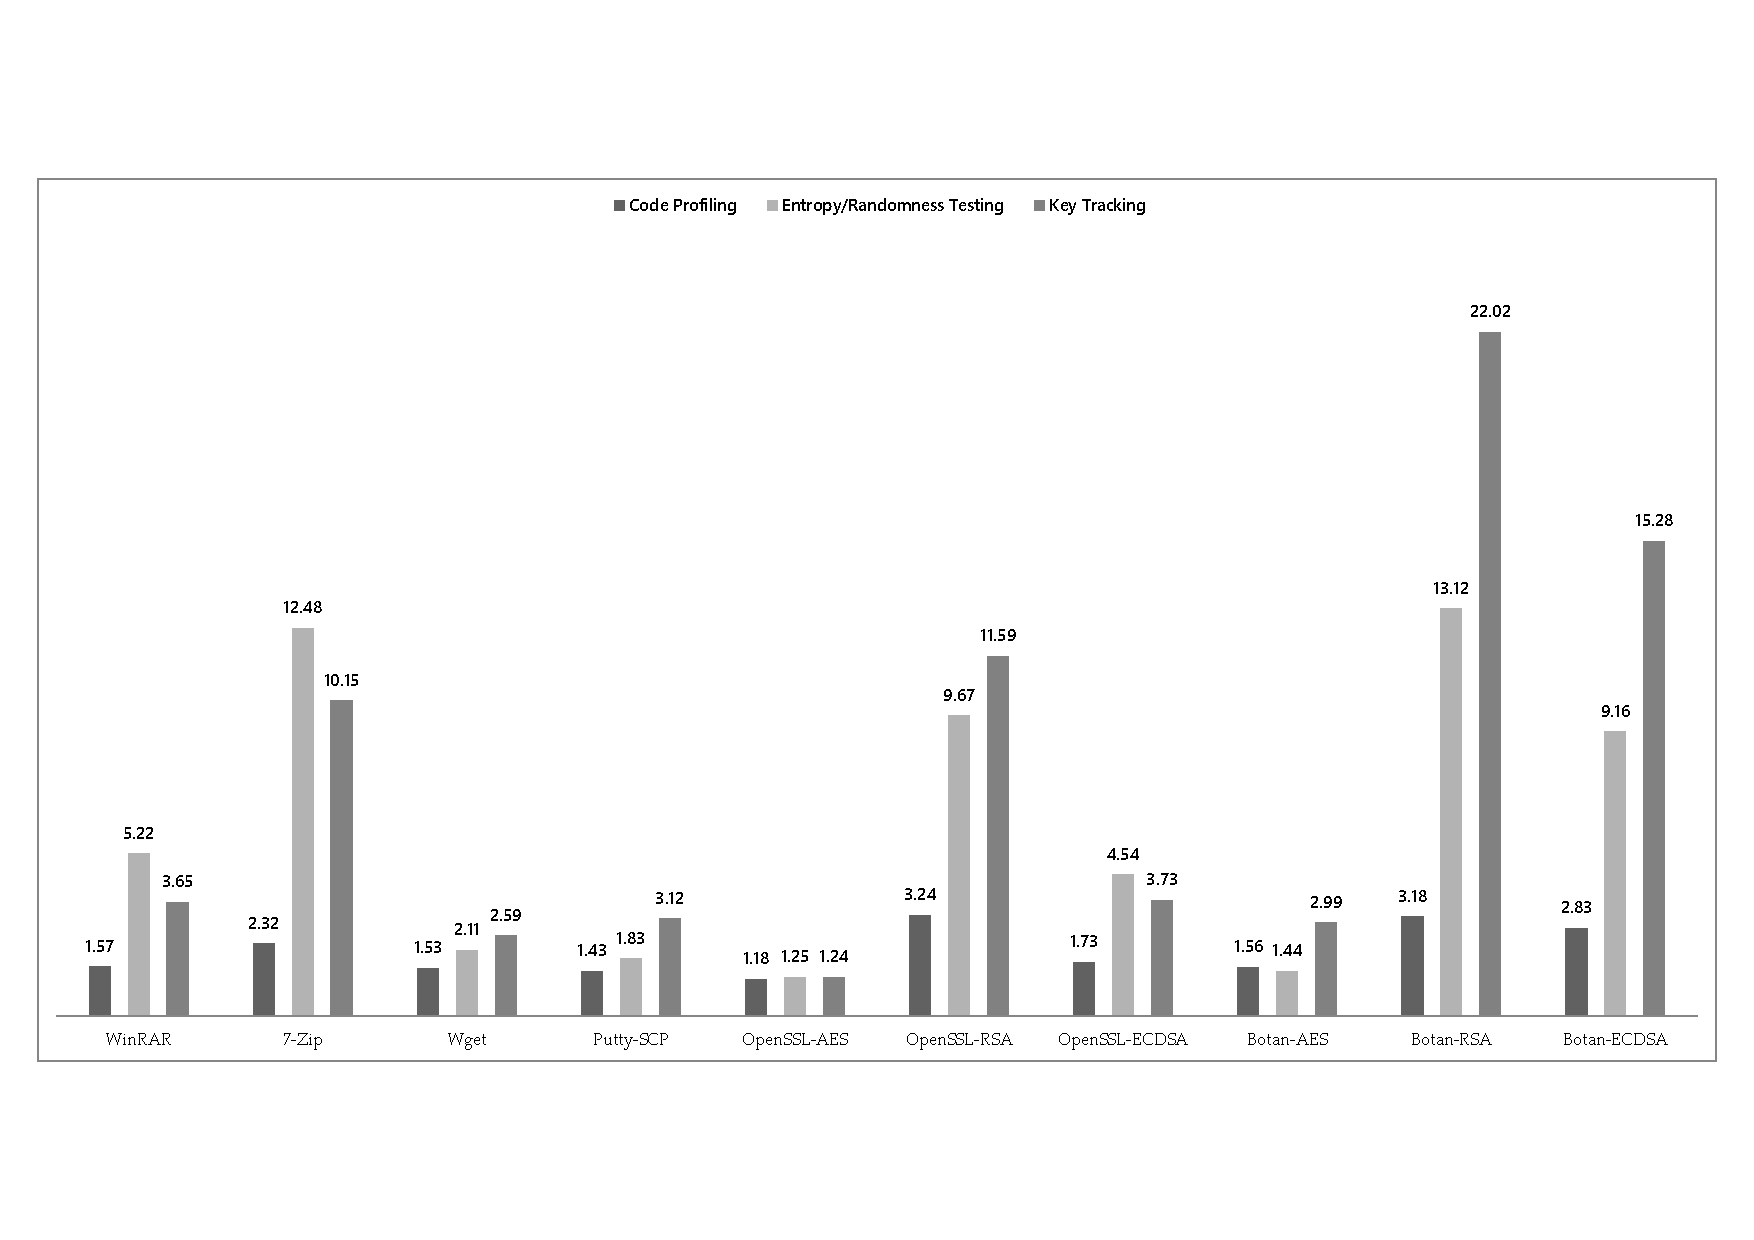
\includegraphics[width=0.5\textwidth]{barg.pdf}
% \caption{Performance overhead\label{fig:perf} }
% \end{figure}

\begin{figure*}
\centering
\resizebox{7.2in}{!}{
\includegraphics[width=1.5*\linewidth]{figure/perf.tikz}
}
\vspace{-0.1in}
\caption{Runtime overhead (times) of three pintools of \sysname compared to null PIN.}
\label{fig:spec:shadowperf}
\end{figure*}

As described in \S\ref{sec:kxray}, \sysname includes three {Pintools}: \emph{code profiling},  \emph{randomness testing}, and \emph{key tracking}. To evaluate the performance overhead of these Pintools, we selected four command-line crypto applications and two representative crypto libraries. 
% to the easier measurement (and no noise) with them. % As shown in Figure~\ref{fig:perf}.
We report the performance overhead of the three Pintools compared to null PIN by running the 6 selected programs 10 times each. As shown in \autoref{fig:spec:shadowperf},
on average the performance overhead of code profiling is 2.1 times, 5.7 times for randomness testing, and 7.6 times for key tracking. We observe that the overhead is larger for programs with complex data transformation (e.g., 7-zip), asymmetric ciphers (e.g., RSA), and digital signatures (e.g., ECDSA). Nonetheless, the performance overhead is reasonable for most programs tested by \sysname. %, and we have not attempted to aggressively optimize its performance.

% To compare the efficiency our approach,
% 	we conducted seven items of testing:
% 	1) \emph{Normal execution}: programs are executed without being analyzed;
% 	2) \emph{Null PIN}: programs are executed with PIN VM but without any instrumentation stub;
% 	3) \emph{Key Pinpointing}: programs are executed with code profiling instrumentor of \sysname;
% 	4) \emph{Key tracing}: programs are executed with code tracing instrumentor of \sysname
% 		(to conduct key tracing with execution sampling, we set the instruction recording threshold to 64);
% 	5) \emph{Dataflow tainting}: programs are executed with our modified version of \emph{libdft}~\cite{kemerlis2012libdft} based on PIN framework to support Windows program;
% 	6) \emph{Data dependency analysis}: recorded traces are analyzed offline with \sysname scripts;
% 	7) \emph{Static Symbolization}: binary executables are statically analyzed by \emph{pysymemu}~\cite{pysymemu} to generate symbolic expression for each function.
% We choose four samples: \texttt{WinRAR}, \texttt{ccrypt}, \texttt{Putty-SCP}, and \texttt{Wget} in \textsc{CryptoZoo}.
% For dynamic analysis,
% 	\texttt{WinRAR} and \texttt{ccrypt} were executed to deal with an input file of 1MB,
% 	while \texttt{Putty-SCP} and \texttt{Wget} were executed to download a 1MB file from a local Linux server.
% To evaluate the efficacy of dynamic program analysis,
%     we also set a terminating condition for each program:
%     if the overhead of one testing exceeds to 10,000 times of the original raw execution,
%     or the network connection is time out, the testing is terminated.



%We also tested the execution time of \sysname. In our experiments, \sysname successfully instrumented all test targets and finished the analysis within several minutes to several hours according to the size of the target program. The most time-consuming stage is the offline taint analysis, which consumes the execution trace and builds data dependency between the key and the inputs. As Table~\ref{tab:insecKey} shows, the size of execution trace varies from xx MB to XX GB. All of them can be recorded without affecting the normal execution of the test target.

% The lightweight key pinpointing slowed down the execution by about 50-100 times.
% The key tracing slowed down each program's execution by about 100-200 times,
% 	and programs such as \texttt{Putty-SCP} can successfully fulfilled network data transferring without suffering from time-out issue.
% By comparison,
% 	dataflow tainting, the prerequisite analysis of many existing approaches, failed to pass each test within a reasonable time.
% For the static analysis part,
% 	since our analysis only deals with the a relatively small size of recorded traces~\footnote{in column 7, size of analyzed tailored trace is listed},
% 	it achieved an average analysis speed of 0.1M/s.
% Even if our analysis tools were implemented in python scripts,
%     the analysis time was less than seven minutes for every case.
% In comparison,
% 	static symbolization methods analyzes the entire program instead of tracing data.
% For programs with moderate size (\texttt{Wget} and \texttt{Putty-SCP}),
%     it spent one or more days to accomplish the symbolization process,
%     and this does not include the latter matching procedure (which we did not implement).



 

\section{Limitations and Future Work}
\label{sec:discussion}
%We have shown that \sysname can be used to detect the insecure crypto keys in real world binary executables. 
%However, 
\sysname %is still not perfect and it 
has a number of limitations. %In this section, we discuss the limitations of \sysname and outline our future work.
%
%
First, while \sysname is able to pinpoint the insecure keys, it does not report any specific crypto algorithms (e.g,. \textsf{\small AES}, \textsf{\small DSA}) to which the insecure key belongs. 
In fact, \sysname has all the building blocks to support the identification of each specific crypto algorithm used by an binary executable. 
More specifically, since \sysname has identified the data bundles of key buffer $K$, ciphertext $C$, and plaintext $P$, we can actually perform a brute force search of the encryption algorithm $E$ by computing whether $C = E (K, P)$, where $E$ are those well-known crypto algorithms. 
Certainly, this is only possible when software uses standard crypto algorithms (e.g., if they follow the never-implement-your-own-crypto practice~\cite{schneier1999cryptography, apvrille2005secure}). 
We leave the identification of specific crypto algorithms in a binary executable as one of our future efforts.

Second, \sysname performs the taint propagation at the function level. 
That is, if a function uses a tainted tag, all the data defined in that function will have that tainted tag. 
Such taint propagation may overly propagate the tainted tag, making insecure keys appear secure. 
For instance, it might be possible that a function uses a random function, but the return value of the random function is never assigned to the crypto key. 
While we have not encountered such a case, we plan to address this issue by implementing a fine-grained taint propagation policy, and meanwhile address the performance issues caused from this policy.

Finally, \sysname will not be able to detect the crypto keys if they are stored in CPU registers. 
A particular case is the secure in-cache execution~\cite{guan2014copker, chen2017secure} technique against the cold-boot attack~\cite{halderman2009lest}.
In this case the crypto key is never evicted to memory and thus our approach is not able to detect it.

There are also other possible extensions of \sysname. 
For instance, crypto operations are increasingly used by mobile apps to protect their sensitive data. Thus, extending \sysname to detect insecure keys in mobile apps is a logical next step. 



%\FloatBarrier

\section{Related Work}
\label{sec:related}
%\vspace{-0.1in}
\paragraph{Crypto Key Identification} There has been significant interests of identifying crypto keys. For instance, Shamir \emph{et al.} presented an efficient algebraic attack which can locate the secret \textsf{\small RSA} keys in long bit strings, and more general statistical attacks which can find arbitrary crypto keys embedded in large programs~\cite{shamir1999playing}. Halderman \emph{et al.} proposed the cold-boot attack~\cite{halderman2009lest} to retrieve the crypto keys from physical memory of the device. Hargreaves \emph{et al.} presented a linear scan method to recover encryption keys from memory~\cite{hargreaves2008recovery}. Maartmann \emph{et al.} discussed the forensic identification and extraction of crypto keys~\cite{maartmann2009persistence}. However, those approaches focus on identifying a key with its mathematic structure and do not consider utilizing dynamic program analysis to discover the used key, whereas \sysname fully utilizes dynamic program execution information such as the number of basic block execution and data entropy/randomness to identify the crypto key. Moreover, \sysname makes a step even further by using the dynamic taint analysis to detect the insecure crypto keys, which is less concerned by previous key identification studies.

\paragraph{Crypto Primitive Identification} A number of efforts have focused on identifying the crypto primitives from various aspects (e.g., ~\cite{grobert2011automated, matenaar2012cis, li2012cipherxray, calvet2012aligot, ruoxu2011detection}).
However, archiving efficient and accurate crypto primitive identification is still a non-trivial task. 
There are still many open challenges needed to be addressed. Recent results indicate that data flow analysis~\cite{lestringant2016assisted, lestringant2015automated} is a promising technique to help identify crypto algorithms. 
One major problem of state-of-the-art crypto primitive identification techniques is that they are sensitive to function boundary and parameter recognition. Existing techniques (e.g., CryptoHunt~\cite{xu2017cryptographic}) require the boundary of crypto function to be identified accurately to recognize crypto function. %Then static or dynamic analysis is employed to build a fine-grained description of either syntactical or semantic feature of the analyzed target. However, crypto algorithm is often not ideally implemented within an independent function but often inextricably interweaves with code of other functionalities. Thus the identification cannot be very accurate inherently. 
% In comparison, our approach uses dynamic analysis to precisely recognize the function boundary, and there is no need to identify function parameters in \sysname.% does not have to identify the parameters of the used crypto function precisely, but focuses on identify the used key instead.


\paragraph{Crypto Misuse Detection} 
Public awareness of crypto flaw is growing and the increased awareness has resulted in an increase of efforts to detect crypto misuses~\cite{lazar2014does, duong2011cryptography, li2014icryptotracer}. 
Over the past a few years, many crypto misuse cases in mobile apps and firmwares (e.g.,~\cite{egele2013empirical, costin2014large}) have been discovered. 
For commodity software,	some crypto misuses for popular software products are also discovered~\cite{wu2005misuse, duong2011cryptography, dodis2013security, everspaugh2014not}. 
{
Recently, TaintCrypt~\cite{rahaman2017program}  proposed the concept of cryptographic program analysis to help developers detect the crypto misuse using LLVM-based static source code analysis.
However, it requires the source code to conduct the analysis.
}
\sysname complements the existing crypto misuse detection approach by exclusively focusing on identifying the insecure crypto keys from binary executables. 


% \paragraph{Dynamic Taint Analysis} Chow \emph{et al.} presented TaintBochs~\cite{chow2004understanding}, a simulator that can track tainted data through an entire system. They investigated the data lifetime of sensitive information (e.g., password) in several commonly-used applications. Since then, dynamic taint analysis has been widely used in many security applications, such as exploit detection~\cite{song2005ndss}, protocol reverse engineering, data structure reverse engineering, malware analysis, so on and so forth. \sysname extends dynamic taint analysis with new applications of insecure crypto key discovery.

%Quantitative information flow analysis~\cite{mccamant2008quantitative, newsome2009measuring} is a technique to evaluate the security of the program. Specifically, it produces an upper bound of the amount of information leaked by a program at runtime. Our adopted key lifetime analysis is a specialized information flow analysis focusing on crypto key audit.  
\def\semicheck{\checkmark\kern-1.1ex\raisebox{.7ex}{\rotatebox[origin=c]{125}{--}}}


\newcommand{\tickYes}{\ding{51}}
\newcommand{\tickNo}{\ding{55}}

\begin{table}[t]
\scriptsize
\begin{tabular}{r llllllll} %\hline

\hline
		\textbf{Systems} & C1 & C2 & C3 & C4 & C5 & C6 & C7 & C8 \\
\hline

	\textsf{Aligot}~\cite{calvet2012aligot}				& \tickNo	& \tickYes	& \tickYes	& \tickYes	& \tickYes	& \tickNo	& \tickYes	& \tickNo	\\ %Done
	\textsf{CipherXRay}~\cite{li2012cipherxray}			& \tickYes	& \tickYes	& \tickYes	& \tickYes	& \tickYes	& \tickYes	& \tickYes	& \tickNo	\\ %Done
	\textsf{Crypto-DFG}~\cite{lestringant2015automated}	& \tickNo	& \tickNo	& \tickYes	& \tickYes	& \tickYes	& \tickYes	& \tickNo	& \tickNo	\\ %DONE
	\textsf{Cryptohunt}~\cite{xu2017cryptographic}		& \tickNo	& \tickYes	& \tickYes	& \tickYes	& \tickYes	& \tickYes	& \tickNo	& \tickNo	\\ %DONE
	\textsf{Dispatcher}~\cite{caballero2009dispatcher}	& \tickYes	& \tickNo	& \tickYes	& \tickYes	& \tickYes	& \tickYes	& \tickNo	& \tickNo	\\ %Done
	\textsf{Kerckhoffs}~\cite{grobert2011automated}		& \tickNo	& \tickYes	& \tickYes	& \tickYes	& \tickYes	& \tickNo	& \tickYes	& \tickNo	\\ %Done
	\textsf{MovieStealer}~\cite{wang2013steal}			& \tickYes	& \tickYes	& \tickYes	& \tickYes	& \tickNo	& \tickYes	& \tickNo	& \tickNo	\\ %DONE
	\textsf{ReFormat}~\cite{wang2009reformat}			& \tickYes	& \tickNo	& \tickYes	& \tickYes	& \tickYes	& \tickYes	& \tickNo	& \tickNo	\\ %Done

\hline
	\sysname									& \tickYes	& \tickYes &  \tickYes &  \tickYes & \tickYes  &  \tickYes & \tickYes & \tickYes  \\ %DONE
 		
 		\hline
 		\\
 \multicolumn{3}{l}{C1: No need of crypto template} &  \multicolumn{6}{l}{C2: Obfuscation resilient}\\
 \multicolumn{3}{l}{C3: Detecting block cipher} &  \multicolumn{6}{l}{C4: Detecting stream key cipher}\\
 \multicolumn{3}{l}{C5: Detecting public-key cipher} &  \multicolumn{6}{l}{C6: Detecting proprietary cipher}\\
 \multicolumn{3}{l}{C7: Identifying crypto key} &  \multicolumn{6}{l}{C8: Detecting insecure key}\\
 \\
\end{tabular}
%\vspace{-0.15in}
\caption{Comparison with the closely related works.}
\label{tab:comparison}
\end{table}

\paragraph{Comparison} Clearly we are not the first to look into the security issues of crypto code, and there are a number of closely related works that focus on identifying the crypto primitives, as shown in~\autoref{tab:comparison}. % To evaluate the effectiveness of our approach, we also compared our \sysname with seven state-of-the-art cryptographic primitive identification systems. The comparison results are listed in Table~\ref{tab:comparison}.
In particular, among the compared systems, \textsf{\small Kerckhoffs}, \textsf{\small Aligot}, \textsf{\small Crypto-DFG}, and \textsf{\small Cryptohunt} require the pre-defined templates to identify crypto algorithms. Therefore, they cannot detect proprietary ciphers. \textsf{\small ReFormat}, \textsf{\small Dispatcher}, and \textsf{\small MovieStealer} are not specifically designed for crypto primitive identification, and thus they cannot identify the crypto keys. Only \textsf{\small CipherXRay} and \sysname can identify both proprietary ciphers and crypto keys, but \textsf{\small CipherXRay} did not make any attempt to identify the insecure keys.
{Moreover, a substantial difference between \sysname and \textsf{\small CipherXRay} is that \sysname focuses on the core part of a crypto algorithm and identifies keys from only several crypto blocks.
In contrast, \textsf{\small CipherXRay} needs to recover both input and output parameters of the entire crypto algorithm.
Thus it still suffers from the issue of how to accurately identify the boundary of parameter buffers and faces both false positives and false negatives~\cite{lestringant2017thesis}.
}
% Meanwhile, all of the previously designed systems did not consider the detection of insecure crypto keys. \sysname is the first system that detects insecure crypto key in binary executables.

An important requirement for the crypto identification is that the analysis should not affect the normal execution of the program.
\textsf{\small ReFormat}, \textsf{\small Dispatcher}, \textsf{\small MovieStealer}, and our \sysname utilize lightweight heuristics, which do not impose much overhead to the normal execution.
\textsf{\small Kerckhoffs}, \textsf{\small Cryptohunt} and \textsf{\small Aligot} use an offline analysis strategy. %: they first record the execution traces and then conduct the time-consuming analysis offline.
\textsf{\small Crypto-DFG} performs a purely static Data Flow Graph (DFG) isomorphism based detection and thus does not affect the execution either.
Only \textsf{\small CipherXRay} adopts a heavyweight dynamic taint analysis and may affect the execution. % More specifically, \textsf{\small CipherXRay} identifies cryptographic operations through the checking of whether the information flow between input and output exhibits an avalanche effect. It also requires to analyze multiple pairs of input-output, and if the input buffer is large, the taint analysis of \textsf{\small CipherXRay} has to maintain many taint tags and thus introduces significant runtime overhead. 
For instance, it takes CipherXRay about 40 minutes to recover a 1024-bit \textsf{\small RSA} private key, which is unacceptable for establishing normal network connection.

We also compared the accuracy of each system.
We found that if the approach requires a very precise criteria to judge the crypto function, it yields false negative.
For instance, \textsf{\small Kerckhoffs} uses I/O comparison with known cryptographic functions to identify specific ciphers.
However, this comparison is very sensitive to the implementation variation. %: if the input/output format of the tested crypto function does not corresponds to that of the template, it cannot be identified even though the test function is a specific crypto algorithm.
Moreover, we also found that only using one heuristic feature to detect crypto algorithm is often not accurate.
\textsf{\small Dispatcher}, for example, has both false positives and false negatives~\cite{matenaar2012cis,grobert2011automated}.
Another case is \textsf{\small CipherXRay}, %It defines the concept of avalanche effect to help identify crypto routines.
%Nonetheless, this concept is not strictly equivalent to the cryptographic avalanche effect: 
which only checks whether all bits of the output buffer are affected by each bit of the input buffer. For the cryptographic avalanche effect, however, the criteria becomes if one bit of the input buffer is flipped, the output buffer changes significantly (e.g., half the output bits flip).
As a result, \textsf{\small CipherXRay} does not check the intrinsic properties of the avalanche effect and may suffer from false positives. In contrast, \sysname focuses on the intrinsic properties of crypto operations, does not require any templates or signatures, and is thus crypto implementation agnostic.
%And \sysname adopts a set of static and dynamic heuristic features to eliminate false positive: if the candidate satisfies all required features, the accuracy of the detection can be proved.

Finally, since binary executables can be obfuscated, the identification of crypto primitives must also consider the code obfuscations. Among the compared systems,  \textsf{\small Dispatcher},  \textsf{\small ReFormat}, and \textsf{\small Crypto-DFG} can be easily cheated by changing the instructions with alternatives and thus are not obfuscation-resilient. 
%For instance, \textsf{\small Dispatcher} labels a function as an encoding one if the function executes a minimum number of instructions (e.g., 20) and has a ratio larger than a pre-defined threshold (e.g., 0.55). %Obviously, code obfuscation can hinder such detection. 
For obfuscation-resilient systems such as \textsf{\small Kerckhoffs}, \textsf{\small Aligot}, \textsf{\small CipherXRay}, and \textsf{\small Cryptohunt}, they are based on semantics of crypto. For \sysname, it utilizes the fact that even if the crypto basic blocks are obfuscated, e.g., certain arithmetic instructions are replaced by other equivalent arithmetic instructions, % such as using \textsf{\small and}, \textsf{\small or}, \textsf{\small not} to replace \textsf{\small xor},  
the runtime features of execution number and high entropy/randomness cannot be removed. Therefore, \sysname can still work against obfuscated crypto code. \looseness=-1






\section{Conclusion}
\label{sec:conclusion}
We have presented \sysname, a dynamic analysis system to identify insecure keys in an input executable. \sysname first pinpoints the crypto keys by leveraging general properties of crypto operations. 
Then, it identifies insecure keys, namely, deterministic generated keys, insecurely negotiated keys, and recoverable keys by tracking how the crypto keys are generated and propagated. 
We have implemented \sysname and tested it with 10 cryptographic libraries and 15 applications that contain crypto operations. 
Our evaluation results show that \sysname pinpoints the crypto keys used by symmetric ciphers, asymmetric ciphers, stream ciphers, and digital signatures.  
More importantly, \sysname discovers insecure keys in 22 out of 25 evaluated programs, including in well-established crypto libraries such as \textsf{\small LibSodium}, \textsf{\small Nettle}, \textsf{\small TomCrypt}, and \textsf{\small WolfSSL}. 
We have responsibly disclosed the vulnerabilities to the affected software vendors and patches are under development.

\section{Availability}
The source code of \sysname and also the tested benchmark will be made public available at \url{https://github.com/gossip-sjtu/k-hunt/}.

\begin{acks}
The authors would like to thank anonymous reviewers for their valuable comments and helpful suggestions. 
The work was partially supported by the Key Program of National Natural Science Foundation of China under Grant No.:U1636217,
	the National Key Research and Development Program of China under Grant No.: 2016YFB0801200.
This research was also partially supported by the Regional Government of Madrid through the N-GREENS Software-CM project S2013/ICE-2731, the Spanish Government through the DEDETIS grant TIN2015-7013-R, and the European Union through the ElasTest project ICT-10-2016-731535.
We specially thank the Ant Financial Services Group for the support of this research within the \emph{SJTU-AntFinancial joint Institution of FinTech Security}.
\end{acks}

\bibliographystyle{ACM-Reference-Format}
\bibliography{ibi}

\end{document}
